\documentclass[11pt,onecolumn]{article}

\usepackage{url}
\usepackage{amsmath,amsfonts,amssymb,mhchem,chemfig}
\usepackage{cases}
\usepackage{setspace}
\usepackage{caption}
\usepackage{textgreek}
\usepackage{authblk}
\usepackage{natbib}
\usepackage[margin=0.75in]{geometry}
\usepackage[margin=0.5in]{caption}
\captionsetup[figure]{font=footnotesize,labelfont=footnotesize}
\pagestyle{plain}
\providecommand{\keywords}[1]{\textbf{\textit{Key words --- }} #1}
\renewcommand{\abstract}[1]{\textbf{Abstract --- } #1}
%\jshort{mst}

%\volname{}

%\jvolume{0}

%\jvol{}

%\jissue{0}

%\pubyear{2020}

%\mstype{Article}

%\artid{012}

%\access{}
\renewcommand{\baselinestretch}{1.5} 

%\captionsetup{font={stretch=3}}
\newcommand{\othercaption}[1]{\caption{\setlength{\baselineskip}{1.5\baselineskip}#1}}

\begin{document}

\title{Resource uptake and the evolution of moderately efficient enzymes}
\date{\today}
\author[,1]{Florian Labourel\thanks{Corresponding author: \texttt{florian.labourel@univ-lyon1.fr}}}
\author[1]{Etienne Rajon}

 
\affil[1]{Univ Lyon, Université Lyon 1, CNRS,
    Laboratoire de Biométrie et Biologie Evolutive UMR5558,
    F-69622 Villeurbanne, France}

  \maketitle
  
    \abstract{Enzymes speed up reactions that would otherwise be too slow to sustain the metabolism of self-replicators. Yet, most enzymes seem only moderately efficient, exhibiting kinetic parameters orders of magnitude lower than their expected physically achievable maxima. Here, we question how these parameters evolve using a mechanistic model where enzyme efficiency is a key component of individual competition for resources. We show that kinetic parameters are under strong directional selection only up to a point, above which enzymes appear to evolve under near-neutrality. A majority of kinetic parameters compiled elsewhere do spread onto this plateau. Nonetheless, using a population genetics model that includes genetic drift and mutational biases, we show that this is a very unlikely outcome of evolution on a common landscape, as even very moderate biases towards lower efficiency should prevent the occurrence of such a diversity. Instead, differences between species, and within a species between metabolic pathways and the reactions to perform, should be involved. Our results point to drift playing an important role, along with the kinetics of nutrient transporters, the tolerance to high concentrations of intermediate metabolites, and the reversibility of reactions. Enzyme concentration also shapes selection on kinetic parameters, suggesting that the joint evolution of concentration and efficiency, facilitated by the plateau, should matter. Interestingly, the position of an enzyme along the metabolic pathway is not key for its evolution, contrasting with the prediction of models assuming that fitness depends on a precise level of flux control, rather than on competitive abilities.}

\keywords{Enzyme kinetics, $K_M$, $k_\text{cat}$, Membrane transport, Facilitated diffusion, Michaelis-Menten}
\vspace{0.5cm}

%%% Il faut mettre des mots-clés pas trop évidents et pas présents dans l'abstract / le titre
\section{{Introduction}\label{sec:Intro}}

%\vspace{-0.5cm}
Living organisms need to uptake nutrients and metabolize them, relying on enzymes to catalyze chemical reactions along metabolic pathways. Accordingly, and despite being intrinsically reversible \citep{Haldane30,Klipp94}, \textit{in vivo} enzyme-catalyzed reactions are commonly thought of as an irreversible two-step process \citep{Bar-Even11,Bar-Even15,MichaelisMenten1913,Johnson11}:
\begin{equation}
\ce{ E + S <=>[k_{f}][k_{r}] ES ->[k_{cat}] E + P },
\label{chemMM}
\end{equation}
where $k_f$ and $k_r$ are the rates of association and dissociation between enzyme and substrate, and $k_\text{cat}$ is the turnover number, that is the rate of formation of the product $P$ from $ES$ complexes. The first part of this chemical equation describes the encounters between the enzyme $E$ and the substrate $S$; the enzyme will be efficient if $ES$ complexes form often and do not dissociate before the substrate has been turned into a product, which is reflected by the constant $K_\text{M}=\dfrac{k_\text{r}+k_\text{cat}}{k_\text{f}}$. The efficiency $v$ of an enzyme -- the rate at which it makes a product $P$ from $S$ -- depends on these two constants through equation (\ref{EquiBHsimp}):
\begin{equation}
v=k_{cat}.[E_\text{tot}].\frac{[S]}{K_\text{M}+[S]},
\label{EquiBHsimp}
\end{equation}
\noindent under the assumption that the concentration $[S]$ is approximately constant and that of $[ES]$ is at equilibrium \citep{MichaelisMenten1913, Briggs25}.
 
At first glance, Natural selection is presumed to optimize enzymatic efficiency by pushing $k_\text{cat}$ upwards and $K_\text{M}$ downwards to universal physical limits. Enzyme efficiencies are for instance limited by the diffusion properties of their aqueous environment, which sets an upper bound of approximately $10^8-10^{10} M^{-1}s^{-1}$ for the ratio ${k_{cat}}/{K_M}$  \citep{Alberty58,Zhou82}.

Nearly optimal enzymes indeed seem to exist, as exemplified by triosephosphate isomerase (TIM) whose ratio is close to this theoretical ceiling \citep{Knowles77}. But they are uncommon: most enzymes appear to be only moderately efficient and far off these physical limits -- including enzymes immediately flanking TIM in the glycolysis metabolic pathway \citep{Davidi18}.
Indeed, \citet{Bar-Even11} have analysed a dataset of several hundreds of enzymes and found a wide diversity among enzyme parameters, thus sketching a puzzling pattern that has far more in common with a zoo than it looks like variations around an archetypal form. 

To date, three sources of explanations have been invoked to explain both this variance in parameter estimates and the fact that many look suboptimal: (1) \textit{in vitro} estimates do not reflect the \textit{in vivo} functioning of enzymes, (2) physical constraints vary between enzymes such that their achievable optima differ, and (3) Evolution fails to produce optimum properties.

Surely, differences between enzyme behavior \textit{in vivo} and \textit{in vitro} are expected, first because diffusion in a test tube is hardly comparable to diffusion in the cytoplasm \citep{Ellis01,Rivas04,Zhou08,Rivas18}. As the cytoplasm gets packed, the cell approaches a state where molecules are less mobile, hindering substrate-enzyme encounters \citep{Muramatsu88,Zimmerman93,Blanco18}. In this regard, $K_\text{M}$ values are thus underestimated \textit{in vitro}, and enzymes should perform less efficiently \textit{in vivo}. Simultaneously, macromolecular crowding can sometimes improve catalytic activity \textit{in vivo}, making specificity constants $k_{cat}/K_M$ higher than their \textit{in vitro} estimates \citep{Ralston90,Ellis01,Jiang07,Pozdnyakova10}. These effects are obviously important for our understanding of enzyme evolution but do not alone provide a reasonable explanation to the reported patterns insofar as some of them should be partially correlated between enzymes \citep{Tabaka14}, and their reported estimates are rather weak \cite{Davidi16}.

Besides the diffusion limit already mentioned, constraints on enzyme evolution also include an intrinsic trade-off that originates from the dependency of both $k_{cat}$ and $K_M$ on intermediate energy profiles
\citep{Heinrich91}. Nonetheless, this trade-off is scarcely observable among evolved enzymes -- \citet{Bar-Even11} report a coefficient of determination around $0.09$ for the correlation between $\log_{10}(k_\text{cat})$ and $\log_{10}(K_M)$ -- suggesting that it can be overcome. 
Other constraints may exist and be specific of a given reaction \citep{Klipp94} -- \textit{e.g.} reaction reversibility -- potentially explaining a part of the variance in enzyme efficiencies.
Estimating constraints on all individual enzymes appears like a daunting task, which could be guided, in part, by the identification of deviations from evolutionary predictions.

Enzyme evolution has often been considered theoretically through the lens of flux control \citep{Burns85,Fell92,Kacser95}. Indeed, \citep{Kacser73} along with \citep{Heinrich74} brought to light that the control of the flux in a metabolic pathway is shared between all enzymes, in what is known as the summation theorem. Thence, because the sum of control coefficients must equal 1 within a pathway, if all enzymes have similar kinetic parameters, none of them exerts a strong influence. But if one enzyme departs from this trend and becomes inefficient, it exerts a strong control at the expense of others. This leads to diminishing-returns epistasis because, as an enzyme becomes more efficient, subsequent mutations have smaller effects \citep{Kacser73,Dykhuizen87,Tokuriki12}, a finding that have since received empirical confirmation \citep{Fell92,Lunzer05}.

\citep{Hartl85} have considered such a fitness landscape under a population genetics framework to conclude that enzymes may be evolving on nearly neutral landscapes \citep{Ohta92}. More recently, based on similar evolutionary models and a fitness function coming from flux balance analysis, \citet{Heckmann18} have furthered the idea, compellingly showing how diminishing returns epistasis could generate the wide expected variety of $k_{cat}$s at the level of an organism. In these models as in most, an enzyme's efficiency is captured by its activity, generally represented by a composite of $k_\text{cat}$, $K_M$ and enzyme concentration \citep{Hartl85,Kaltenbach14}, such that the distinct evolutionary dynamics of these parameters is ignored.

Perhaps more importantly, \citep{Heinrich91} and \citep{Schuster08} have pointed out that these frameworks assume a constant value for either or both concentrations of the first substrate and of the final product \citep{Orth10}, whereas Evolution should instead maximize the amount of final products generated. \citep{Klipp94} found that the aforementioned concentrations indeed have a major influence on optimal rate constants under certain assumptions. 
Likewise, nutrient uptake is most often not considered explicitly in existing models of enzyme evolution, while it is obviously critical in the competition for resources. 

Nutrient uptake occurs when metabolites move inwards across cell membranes; it may rely on membrane permeability only (passive diffusion) or involve channels and carrier proteins, be they transporters or cotransporters \citep{Stein86a}.
Here we build a model that explicitly includes passive (PD hereafter) or facilitated diffusion (FD) followed by an unbranched metabolic pathway to study how resource availability coupled to transport modulates the evolution of enzymes along the pathway.
In ecological scenarios where individuals compete for resources, Natural Selection should favour genotypes that maximize the net intake of molecules and their transformation, which are linked under both PD and FD. Based on this premise, we show that the evolution of the first enzyme's kinetic parameters $k_f$ and $k_\text{cat}$ takes place on cliff-like fitness landscapes where a fitness plateau covers a wide part of the relevant parameter space. Kinetic parameters have co-dependent but distinct evolutionary dynamics -- and thus distinct sensitivities to certain parameters of the model -- such that the shape of the plateau can be modulated by changing parameters of the model within realistic ranges.

We further show that most empirical estimates for kinetic parameters compiled by \citet{Bar-Even11} are spread on the fitness plateau of a generic fitness landscape. But we also demonstrate, using a simple population genetics model, that this is a highly unexpected evolutionary outcome when we introduce biases -- even very mild -- for the mutations of kinetic parameters. We thus explore the effect of several parameters that may make the fitness landscape of each enzyme unique, thus explaining, at least in part, their exceptional diversity.

\section{Results\label{sec:Results}}

\subsection{Passive diffusion is generally inadequate to sustain cell metabolism}

In the version of our model in which intake relies on passive diffusion (PD), the net uptake of a nutrient is a direct outcome of its concentration gradient, and therefore of how efficiently the first enzyme catalyses its transformation inside the cell. Assuming that fitness is proportional to the flux of product of this reaction, we find that the fitness landscape has a cliff-like shape with fitness increasing steeply as parameters $k_\text{cat}$ and $k_f$ increase (see Supplementary materials, section Text S1). The precise shape will not be commented in detail here, for it is very similar to landscapes obtained under facilitated diffusion (FD, treated in the rest of this manuscript). 

Importantly, our results indicate that PD can only sustain a small part of the metabolism of most living cells given cell permeabilities reported in the literature \citep{Wood68,Milo10}, suggesting that this process may not be a determining factor in the evolution of enzymes along metabolic pathways. Indeed, even extremely efficient enzymes, harbouring values of $k_\text{cat}$ and $k_\text{cat}/K_\text{M}$ close to their physical limits, yield low inward fluxes that approach $10^{-2}~mM.s^{-1}$ when considering a spherical cell with a diameter $D=1 \mu m$. To get a sense of how low these fluxes are, we calculated the maximum cell size that they can theoretically sustain. Considering that basal metabolic demands are approximately proportional to the cell volume and using estimates by \citet{Lynch15} for this relationship, we predicted the maximum size enabled by sugar passive diffusion (see \ref{sec:M&M}Materials and Methods). Setting a (conservatively high) medium concentration in glucose $[G]=1$M yields a theoretical volume ceiling $V_{est}=0.84 \mu m^3$. 

Nearly all eukaryotes, and most prokaryotes are \textit{de facto} larger than this threshold \citep{Heim17}, which might help explain the apparent ubiquity of FD. While this demonstration hinges on numbers for sugar uptake, which may arguably be the task requiring the highest flux, PD may be limiting for many other metabolites \citep{Boer10}, depending on their permeability and availability in the environment: even for very high amino-acids concentrations that may only be met in multicellular organisms \citep{Schmidt16} and assuming the highest observed permeability for such metabolites \citep{Chakrabarti94}, these levels are orders of magnitude lower than with FD (see Supplementary material - section Text S1 for PD results). 

Our calculations therefore suggest that primordial cells, preceding the evolution of FD, must have been extremely small. Current-sized cells, however, must predominantly rely on FD when concentration gradients can be maintained, and on active transport otherwise. 

\subsection{General shape of the fitness landscape under facilitated diffusion}

For most metabolites, FD relies on the specific binding of the substrate to transmembrane carrier proteins (transporters hereafter), followed by its translocation to the other side of the membrane \citep{danielli1954,Kotyk67,Stein86d}. Our model builds on \citet{Kuile94}'s approach to model FD, considering the simplifying assumption of symmetric transport. Within this framework, FD operates on the concentration gradient and is susceptible to saturation, represented by constant $K_T$ -- similar to $K_M$ in the Michaelis-Menten equation -- and an interaction constant $\alpha$ (see Methods for details). We assessed how this saturation phenomenon influences the selection pressure acting on forward enzyme kinetic parameters ($k_f$ and $k_\text{cat}$) under various scenarios. 

\begin{figure*}[t!]
\centering
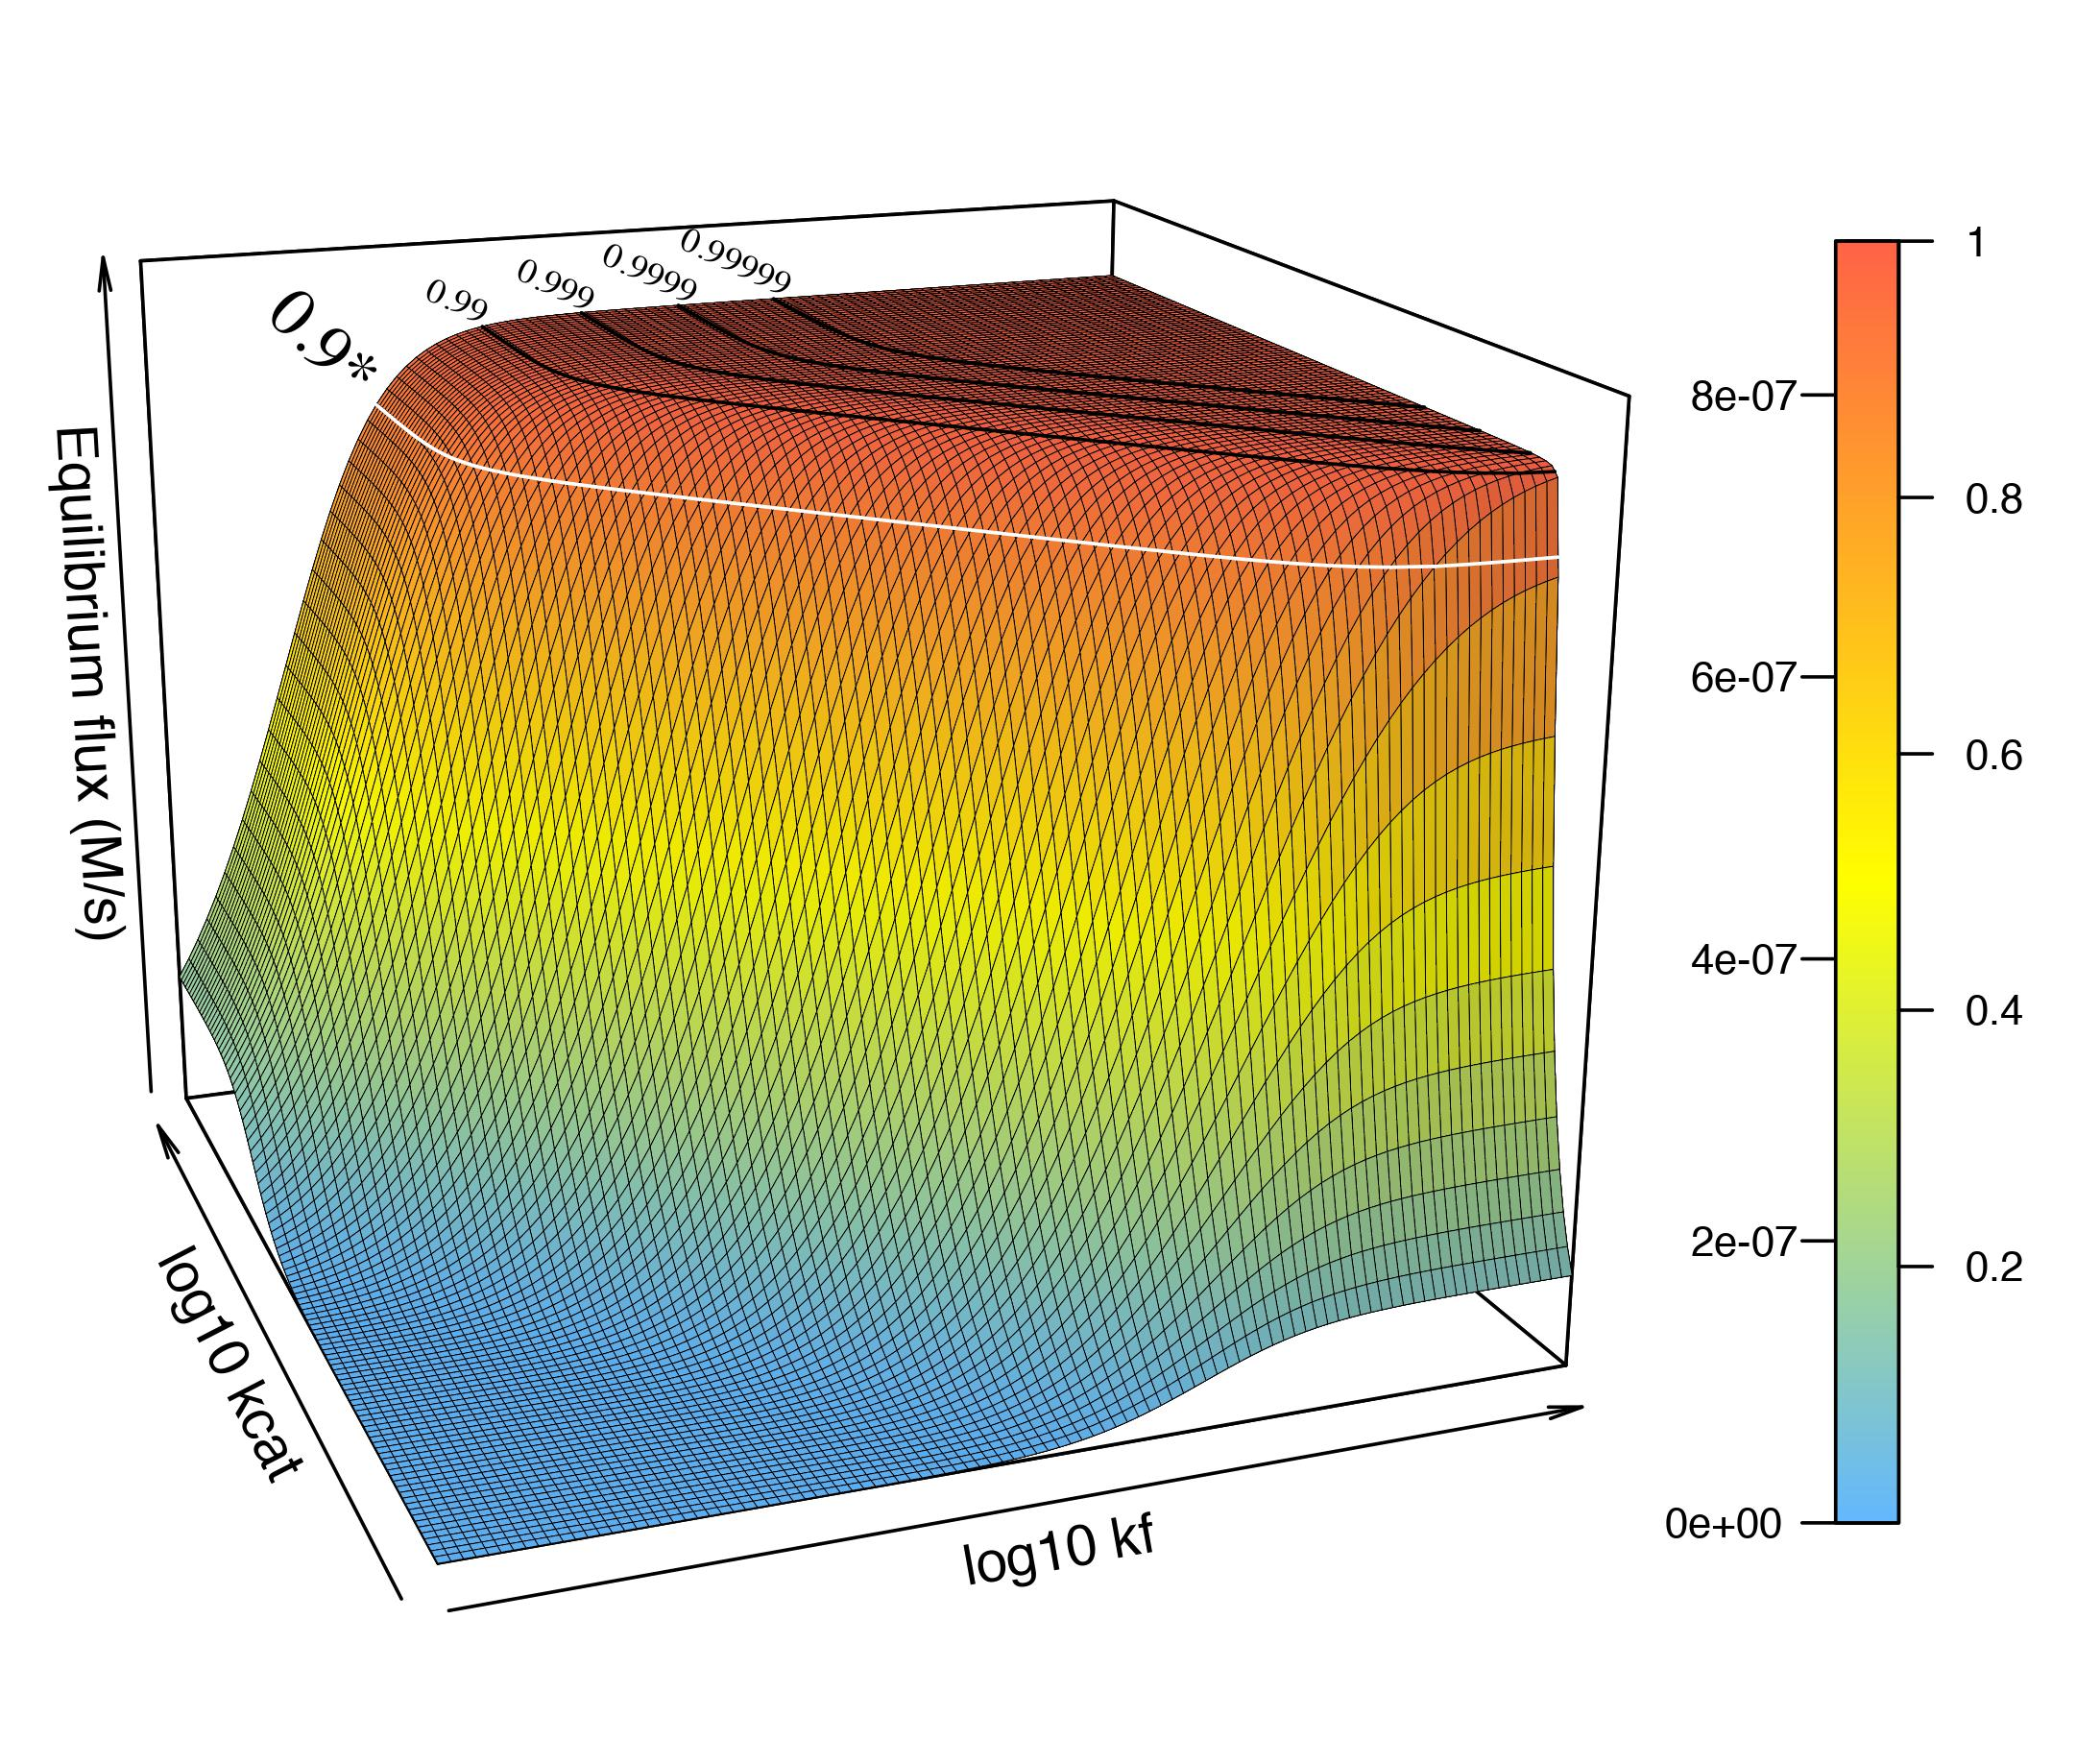
\includegraphics[scale=0.47,trim=0cm 0.75cm 0 1cm,clip]{Figures/3DFitLandscape.jpeg}
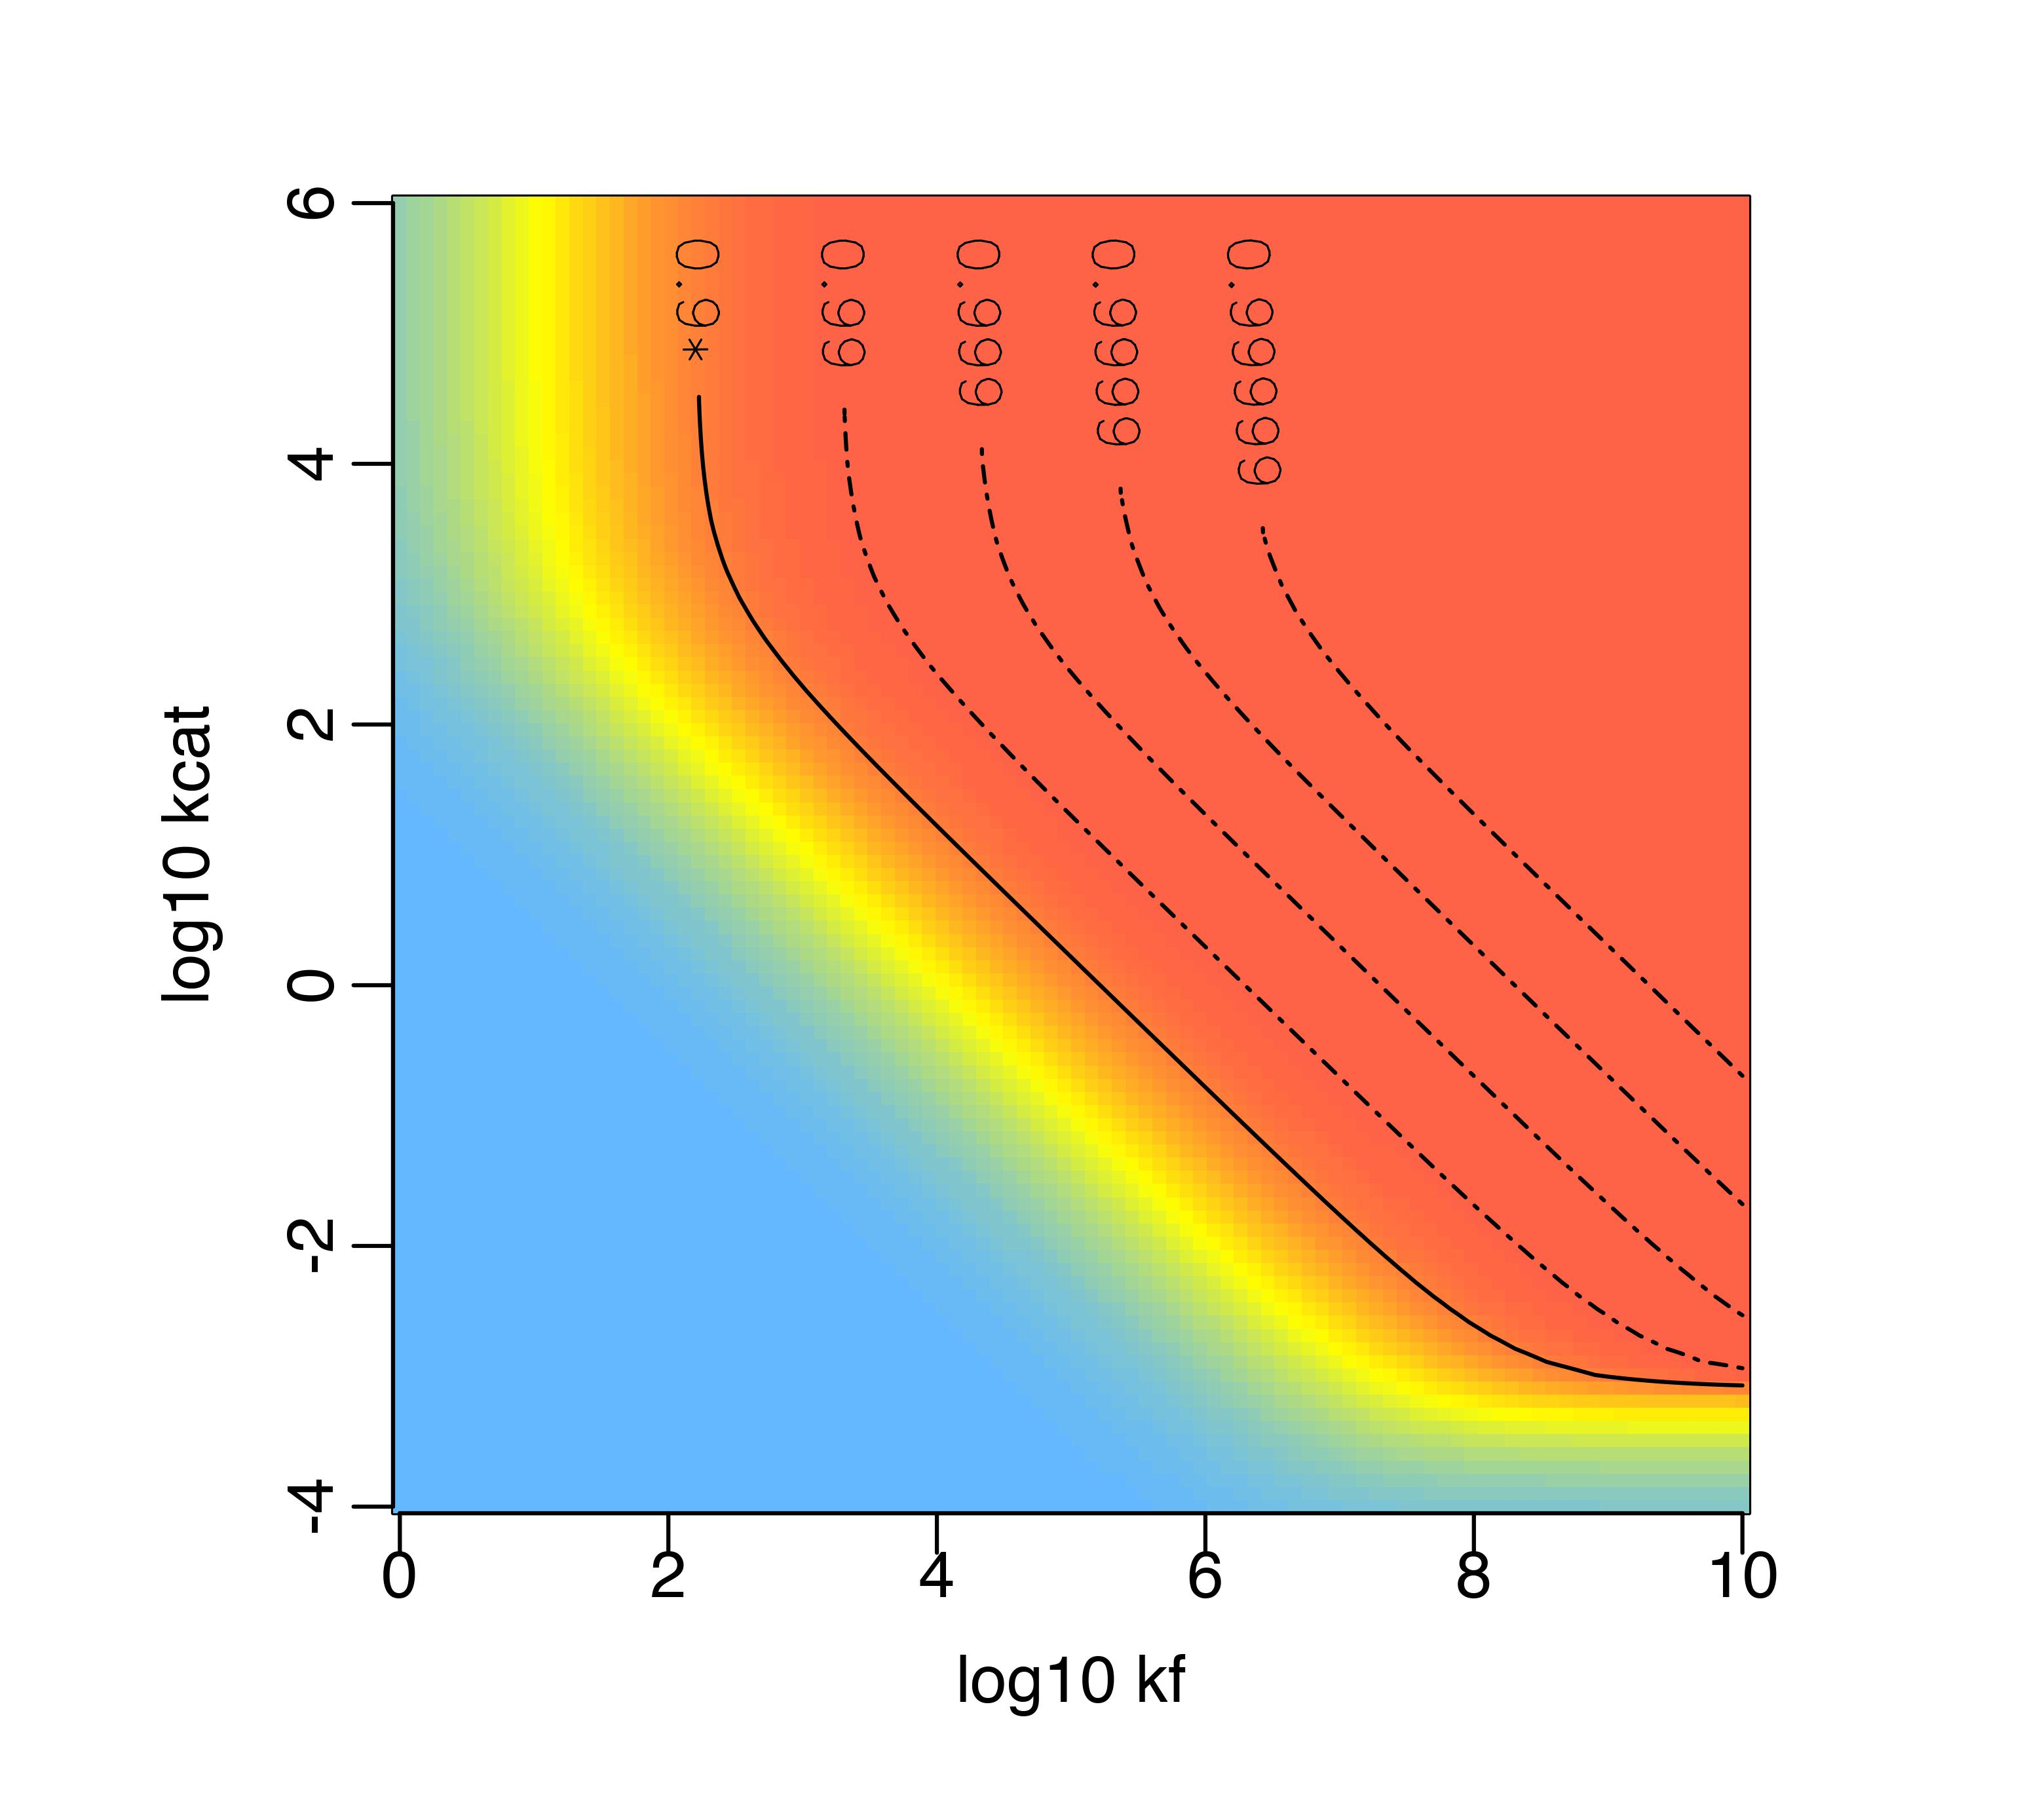
\includegraphics[scale=0.42,trim=0 0cm 0cm 1cm,clip]{Figures/2DFitLandscape.jpeg}
\caption{The flux of product following substrate uptake by transporters and conversion by a dedicated enzyme depends on the kinetic parameters $k_f$ and $k_\text{cat}$ of the enzyme. This landscape is generic in the sense that we avoid focusing on sugars -- arguably extreme cases in terms of flux intensity -- for a general description, considering a moderate flux at saturation $V_{Tm}=1 \mu M.s^{-1}$ close to those measured for amino acids and nucleosides in E.\textit{coli} \citep{Zampieri2019}. We also set the transport saturation ratio $[S_\text{out}]/K_\text{T}$ to 10 such that the FD process approaches saturation, and high transporter affinity $K_\text{T}=50\mu M$, also in line with estimates for nucleosides \citep{Griffith96,Xie04} (see Material and Methods). Other parameter values include $k_r=10^3s^{-1}$ and $[E_{tot}]=1mM$. The color gradient shows the absolute and normalized (such that the maximum flux equals $1$) values of equilibrium flux.}
\label{figure3D2DFit}
\end{figure*}

In order to depict a fitness landscape representative of an average enzyme, we first consider a situation where transporters saturate at an intermediate external concentration of the substrate with an intermediate affinity (FIG.~\ref{figure3D2DFit}). In this situation, the inward equilibrium flux (which, as argued in the introduction, can be considered representative of fitness) forms a plateau when the upstream enzyme in the metabolic pathway has high $k_\text{cat}$ and $k_f$. This low equilibrium flux elasticity coincides with the saturation theory \citep{Wright34, Kacser73}, especially with its version incorporating facilitated diffusion \citep{Kuile94}. The flux plateau is delineated by parallel isoclines (solid and interrupted lines in FIG.~\ref{figure3D2DFit}) oriented in the bottom-right direction of the landscape for intermediate values of $k_\text{cat}$ and $k_f$, such that decreasing $k_f$ by one order of magnitude can be compensated by a similar increase in $k_\text{cat}$. While this mutual dependency holds even for high $k_f$ values as long as $k_\text{cat}$ is not critically low (\textit{i.e.} when $k_\text{cat}>10^{-3}$), it stops when $k_\text{cat}\geq 10^3$, where increasing $k_\text{cat}$ no longer improves fitness. 
Besides, the influence of $k_\text{cat}$ and $k_f$ is not strictly equivalent, since the increase in flux is more gradual in response to $k_f$. 
 
Furthermore, and contrary to the textbook picture whereby most biological reactions are not limited by diffusion at all \citep{Bar-Even11,Sweetlove18}, increasing an enzyme's association rate $k_f$ – be it through its diffusivity or its binding rate – may still enhance the equilibrium flux when diffusion is substantially faster than catalysis.

\subsection{Properties of facilitated diffusion modulate the landscape}

To explore the effect of FD kinetics on the evolution of enzymes in the metabolic pathway, we studied the influence of  $K_T$ -- the affinity of the transporter for the substrate -- and $V_{Tm}$ -- the maximum transport rate -- still assuming that the substrate is close to saturation ($[S_\text{out}]/K_T=10$). We considered ranges of empirical estimates for sugars (high flux with low to moderate affinity in FIG.~\ref{figure2DSEns}, \citep{Stein86d,Maier02}), nucleosides \citep{Griffith96} and amino acids \citep{Stein86d,Zampieri2019} (weak to moderate flux with moderate to high affinity in FIG.~\ref{figure2DSEns}).   

\begin{figure*}[h!]
\centering
\includegraphics[scale=0.35,trim=0cm 0 0 0,clip]{Figures/Fit_Landscape2D_Sensitivity.jpeg} 
\caption{Both the affinity and rate of a transporter have an impact on the (normalized) flux landscape for upstream enzymes, the black isocline (corresponding to $0.9$) delineates the fitness plateau. Each plot represents the landscape obtained with a pair of values for transporters affinity $K_T$ and saturation $V_{Tm}$. Moving one step to the right means that $V_{Tm}$ increases by 1.5 orders of magnitude -- from $10^{-6}$ (low flux) to $10^{-3} M.s^{-1}$ (high) -- and one step up means that $K_T$ decreases by 2 orders of magnitude, starting at $10^{-1}M$ (low affinity). Increasing $K_T$ extends the plateau only towards the left part of the landscape, allowing enzymes with lower $k_f$ on the plateau, whereas decreasing $V_{Tm}$ extends the plateau in both directions. Other parameter values: $k_r=1000/s$, $[E_{tot}]=1mM$ and $[S_{env}]=10 \times K_T$.}
\label{figure2DSEns}
\end{figure*}

We find that increasing the transport flux $V_{Tm}$ exerts a positive selection pressure on kinetic parameters for the upstream enzyme (\textit{i.e.} for increasing $k_\text{cat}$ and $k_f$). The plateau is shifted accordingly, towards the top-right corner of the landscape, at a distance that corresponds to the magnitude of the change in $V_{Tm}$. Increasing the affinity of the transporter (\textit{i.e.} decreasing $K_T$), however, selects for higher $k_{f}$ (the isoclines are displaced to the right and the fold change is similar to that of $K_T$) but has no visible influence on $k_\text{cat}$, a result that holds regardless of the flux at saturation $V_{Tm}$. 
This specific effect on the affinity of the upstream enzyme is likely due to a competition between the transporter -- which can transport the substrate in both directions -- and the enzyme, which harvests the substrate at a rate that depends on the dissociation constant $K_D=k_r/k_f$. It should be noted that nutrients under lower demands -- \textit{e.g.} amino acids -- are generally less concentrated in the environment, often coinciding with a higher affinity of their transporter. Therefore, the possible combinations of flux and affinity likely occupy a restricted space of possibilities where flux and affinity are negatively linked, which as can be seen in FIG.~\ref{figure2DSEns}-A,E,I results in landscapes that mainly differ by the minimum value of $k_\text{cat}$ on the plateau.

\begin{figure}[h!]
\centering
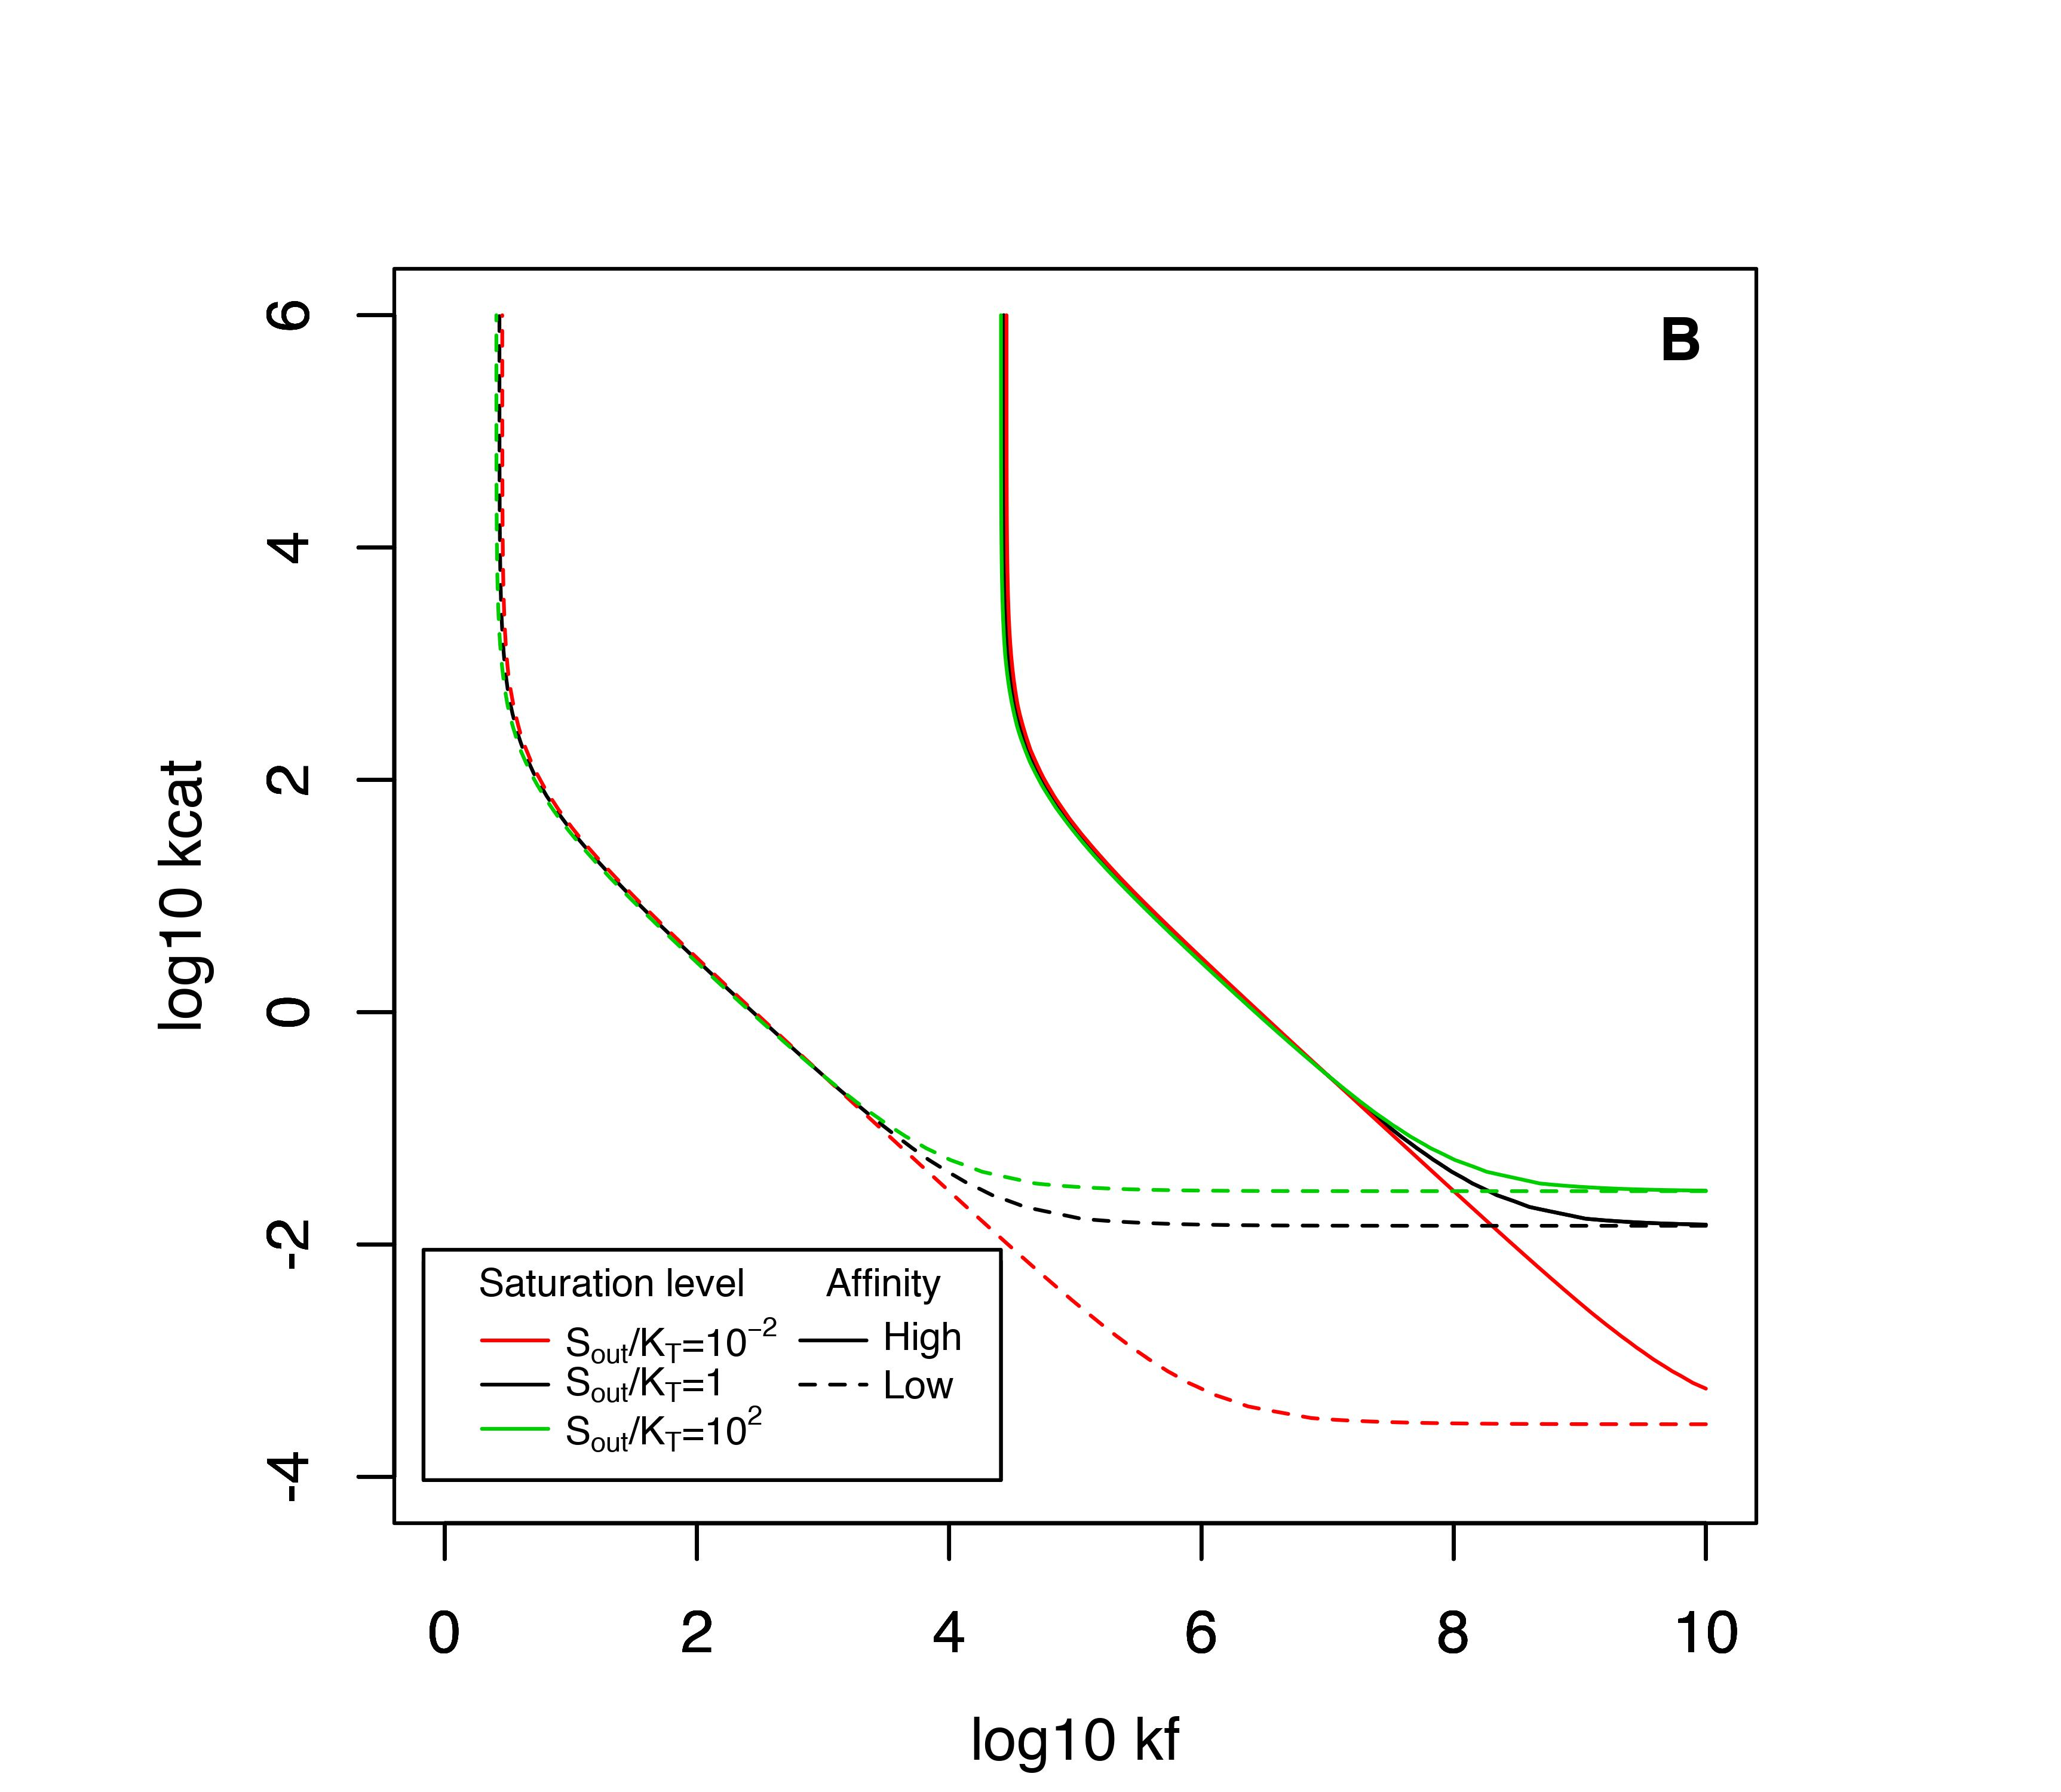
\includegraphics[scale=0.6,trim=0.5cm -0.3cm 0cm 1.5cm,clip]{Figures/2DFit_NonSatToSat.jpeg} 
\caption{The shape of the fitness plateau -- represented for each condition through the $0.9$ isocline (see FIG.~\ref{figure3D2DFit} for details) -- is little dependent on the saturation of the transporter. Only enzymes downstream low affinity transporters show slightly relaxed selection on $k_\text{cat}$ when the external concentration of the substrate is lower than the affinity constant of the transporter, $K_T$. The example shown is for a transporter with moderate flux ($V_{Tm}=10^{-4.5}M.s^{-1}$); the effect is identical for other $V_{Tm}$ (see Figure S2 of SM).}
\label{figure2DSSatStud}
\end{figure}

So far we have considered transporters saturated by high external substrate concentrations. Relaxing this assumption has little impact on the fitness landscape, except that very low values of $k_\text{cat}$ (\textit{i.e.} lower than $10^{-2}$) can   only sustain high fluxes at saturation (see FIG.~\ref{figure2DSSatStud}). Diminishing returns shall thus be the rule for the first enzyme whatever the extracellular environment, and this phenomenon typically occurs within the known behavioral range for both catalysts and transporters.

\subsection{Downstream enzymes also evolve on cliff-like fitness landscapes}

\begin{figure*}[t!]
\centering
\begin{minipage}[c]{0.48\linewidth}
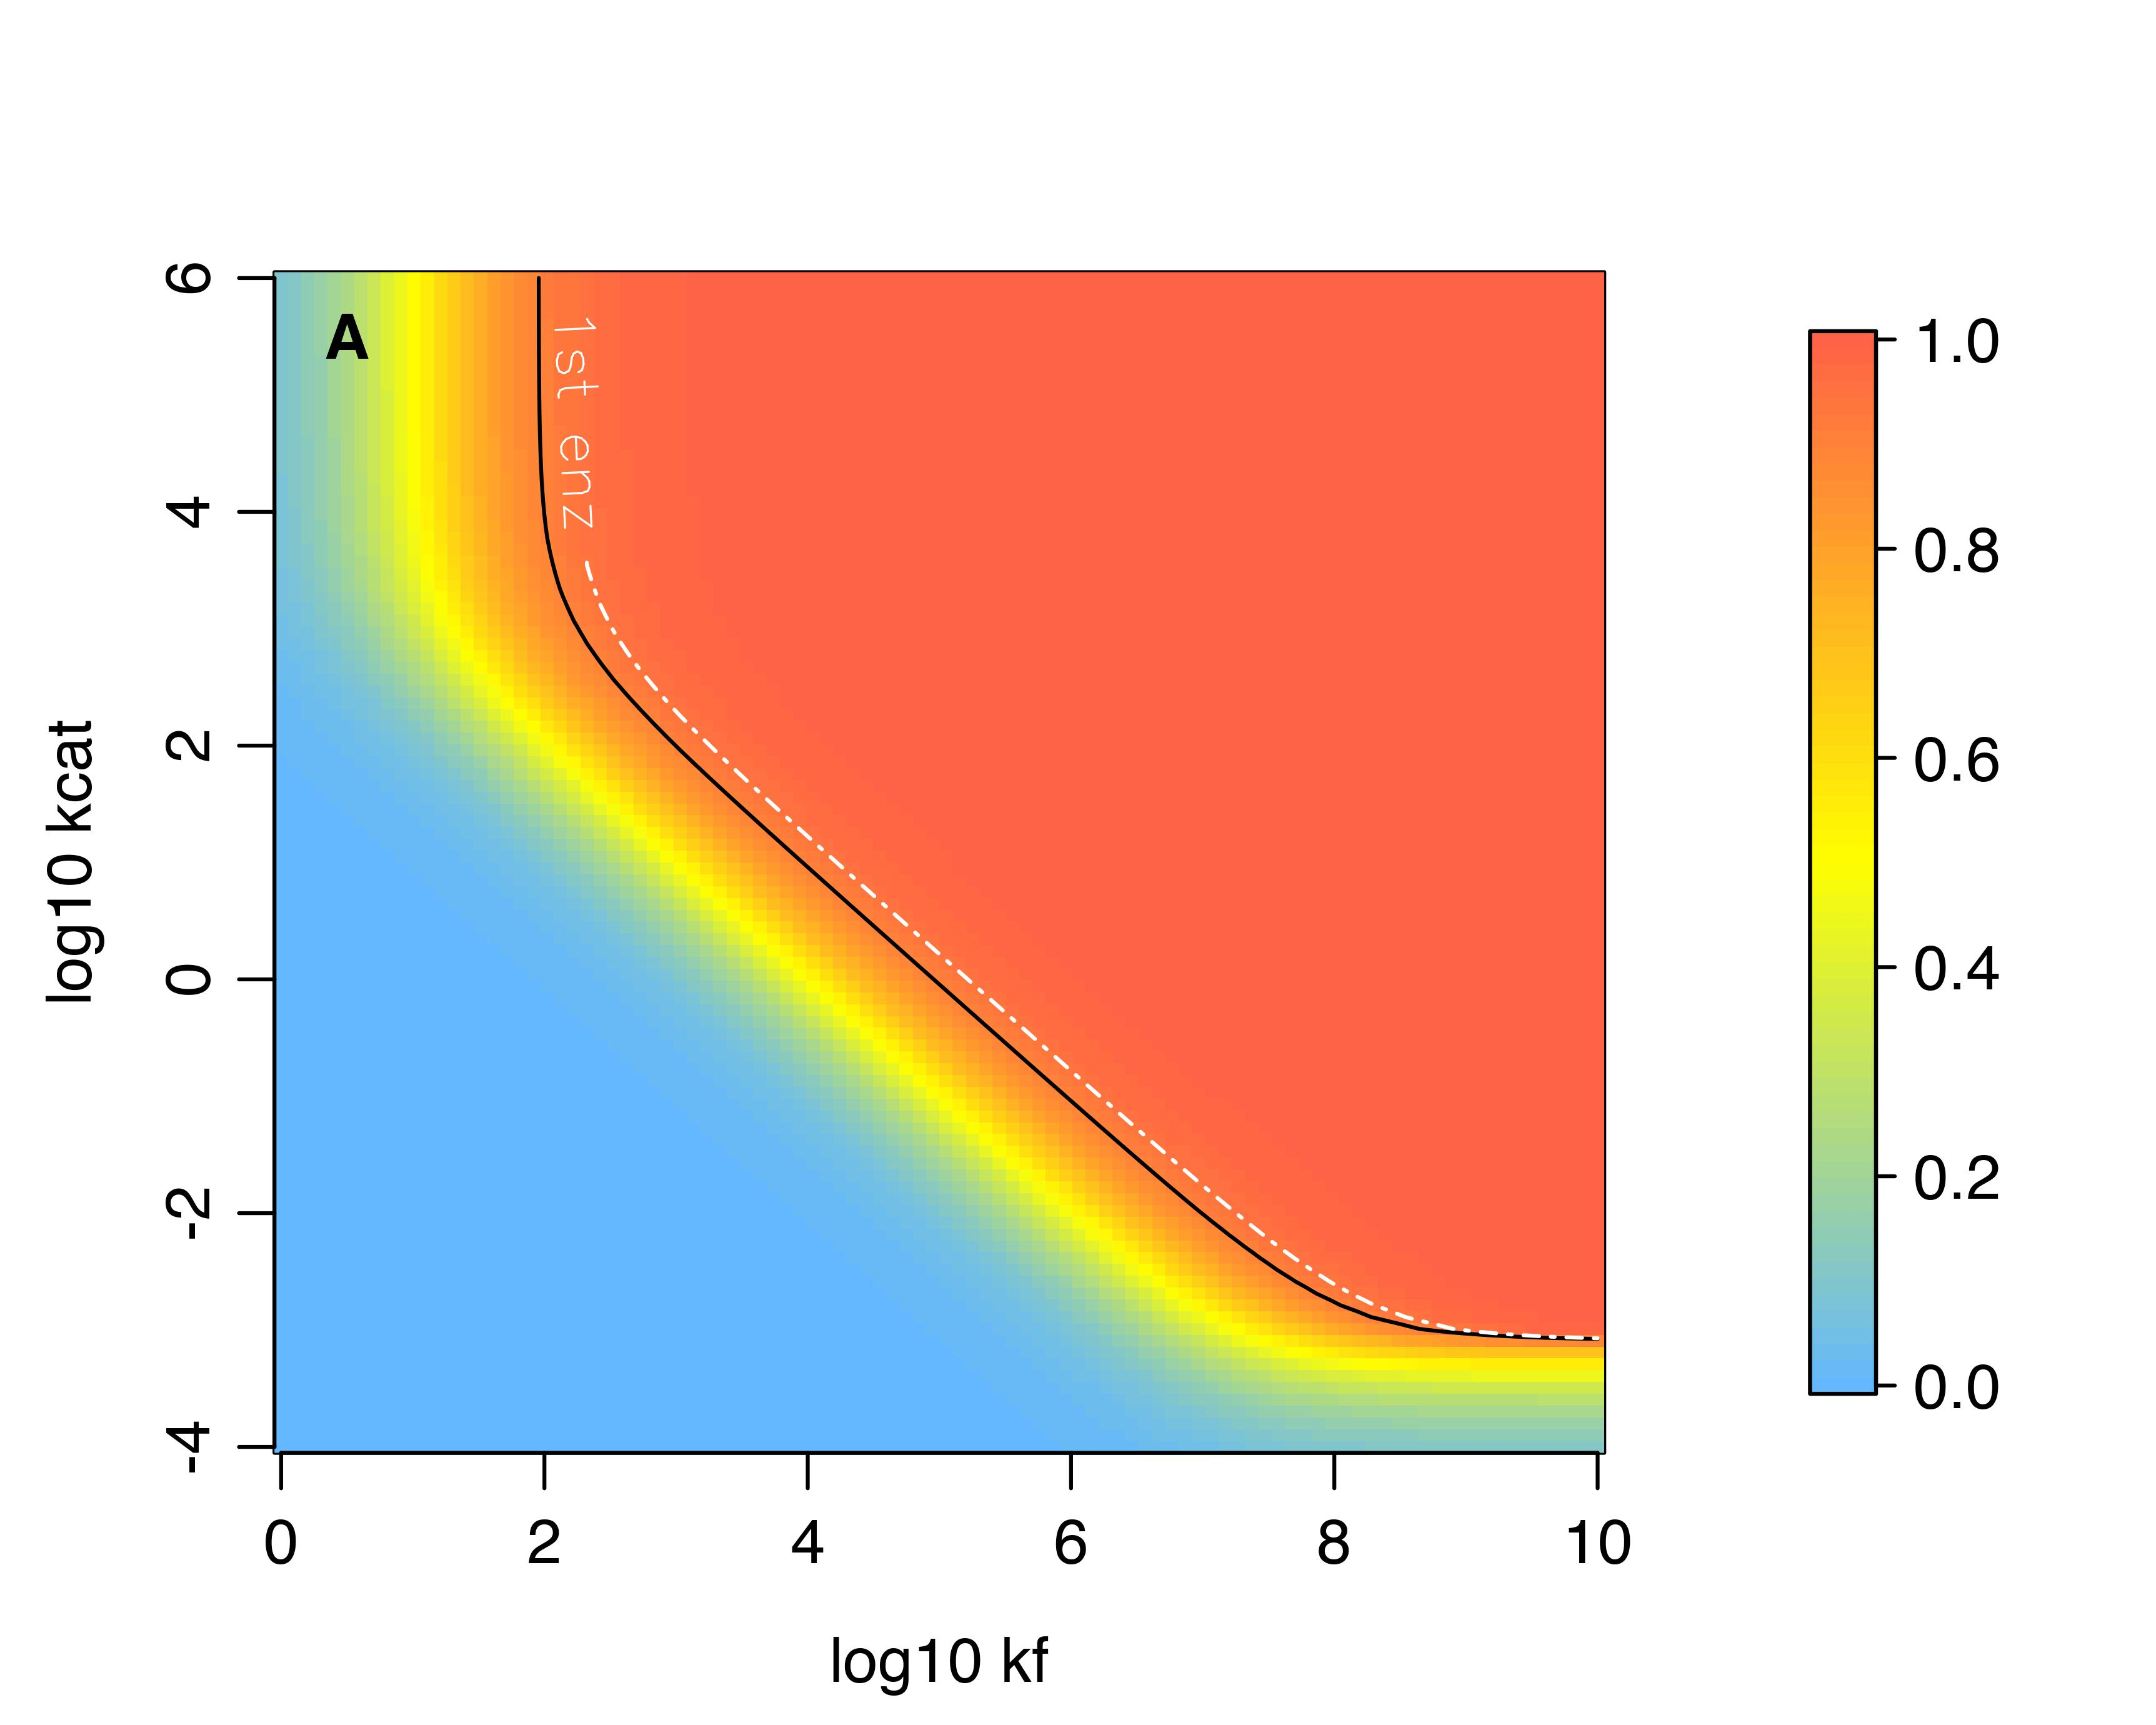
\includegraphics[scale=0.65,trim=0cm 0cm 0cm 1.5cm,clip]{Figures/2DFitLandscape_etahigh_noreverse.jpeg}  
\end{minipage} \hfill
\begin{minipage}[c]{0.48\linewidth}
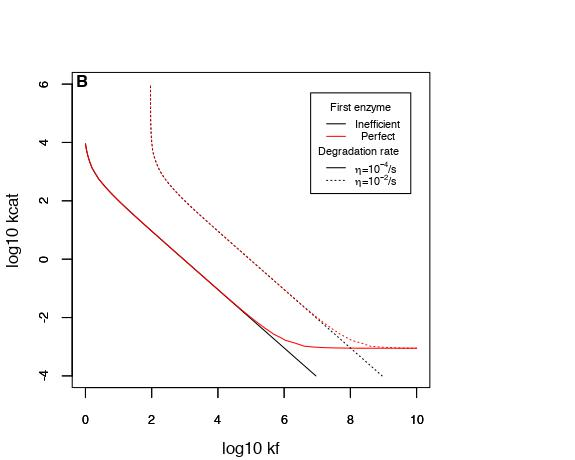
\includegraphics[scale=0.65,trim=0cm 0cm 0cm 1.5cm,clip]{Figures/2DFit_Landscape_2Enz_First_Enz_Influence.jpeg} 
\end{minipage}
\caption{Downstream enzymes exhibit similar fitness landscapes as upstream, with a dependency to degradation parameter $\eta_d$. These enzymes are involved in a moderate flux pathway whose pace is driven by the same uptake kinetics as in FIG.~\ref{figure3D2DFit} where $\displaystyle V_{Tm}=1 \mu M/s$, $\displaystyle K_T=50\mu M$ and $\displaystyle [S_\text{out}]=10K_T$. Settings for the second enzyme also correspond to a model case with $k_r=1000s^{-1}$ and $ [E_{tot}]=1mM$. (A) corresponds to a high degradation rate $\eta_{d}=10^{-1}s^{-1}$ that limits metabolite intracellular concentration to $[S]_{in}=10\mu M$ (for the selected $V_{Tm}$ value), with the upstream enzyme being perfect and concentrated ($k_f=10^{10}M^{-1}.s^{-1}$, $k_{cat}=10^6s^{-1}$, $k_r=10^3s^{-1}$, $[E_{tot}]=1mM$) and results in a fitness landscape very similar to that of the first enzyme when it faces similar conditions (findings are relatively similar for sugar like transporters, as reported in SM - Figure S4), while plateau isoclines drawn in (B) also show results for a second degradation rate limiting this concentration to $[S]_{in}=10mM$, in the context of an upstream concentrated enzyme being either perfect (see above) or inefficient ($k_f=10^{2}M^{-1}.s^{-1}$, $k_{cat}=10^{-2}s^{-1}$, $k_r=10^3s^{-1}$). Decreasing $\eta_d$ makes the cell tolerant to higher concentrations of intermediate metabolites (the product of the first reaction), hence relieving the selection pressure on the second enzyme and moving the plateau towards the bottomleft corner.}
\label{figure2D_2Enz_Deg}
\end{figure*}

In this section, we intend to draw fitness landscapes for enzymes catalysing reactions downstream in the metabolic pathway. Because the flux of the first product in a pathway increases with the substrate gradient across the cell membrane, the upstream enzyme of a given metabolic pathway is selected for efficiency within the limits mentioned in the previous two sections. In contrast, this selective pressure does not apply directly downstream; at steady-state, even inefficient enzymes can in principle process newly formed substrate molecules at an elevated rate, assuming that the concentration of the substrate is allowed to reach any equilibrium value. This is an obviously unreasonable assumption, since a part of this standing substrate should be lost by outward diffusion or degradation, or may interfere with other cellular processes due to the surging involvement in non-specific or promiscuous interactions \citep{Khersonsky10,Schauble13}. We included a degradation term in the model, proportional to the constant $\eta_{d}$ (assuming that the external environment is infinite, the degradation term can as well represent an efflux). Modelling the cost of accumulation this way is likely also consistent with non-specific interactions that should follow Michaelis-Menten kinetics albeit with much lower affinities and rates than the focal reaction, which means their rates should follow a linear relationship up to very high cellular concentrations.

We first consider a ``perfect", highly concentrated upstream enzyme ($k_f=10^{10}M^{-1}s^{-1}$, $k_{cat}=10^6s^{-1}$, $k_r=10^3s^{-1}$, $[E_{tot}]=10^{-3}M$) and study the second enzyme in the pathway, showing that it evolves on a fitness landscape that has a similar shape than described above, still hitting a plateau (FIG.~\ref{figure2D_2Enz_Deg}, with the same parameterization as FIG.~\ref{figure3D2DFit}). The degradation rate creates a ceiling for the concentration of the product of the first reaction, such that reducing $\eta_{d}$ allows for higher concentrations (see SM - Figure S3) and makes the flux tolerant to second enzymes with lower $k_f$s, whereas selection on $k_\text{cat}$ is barely impacted by this parameter. The plateau is therefore extended to the left when high product concentrations are enabled at low $\eta_{d}$ (see FIG.~\ref{figure2D_2Enz_Deg}-B). The shape of the plateau is little impacted by changes in the efficiency of the first enzyme, especially when it stands on the plateau. These conclusions are independent of characteristics of the transporter initiating the pathway, although degradation rates limiting metabolite concentrations to similar levels pushes the plateau to the right slightly more when compared to the landscape of the first enzyme (see SM - Figure S4 for the case of low affinity - high flux transporters). We can notice that the second enzyme's kinetic parameters evolve in response to the net rate $v$ of the upstream reaction and to the presence of any process in competition for its product (like efflux or degradation), such that these results are expected to hold for any enzyme downstream.

\subsection{Most enzymes lie on the fitness plateau}

\begin{figure*}[h!]
\centering
\includegraphics[scale=0.43,trim=0cm -0.75cm 0cm 1.5cm,clip]{Figures/2DFitLandscape_Full_Dataset.jpeg}
\hspace{-0.3cm}
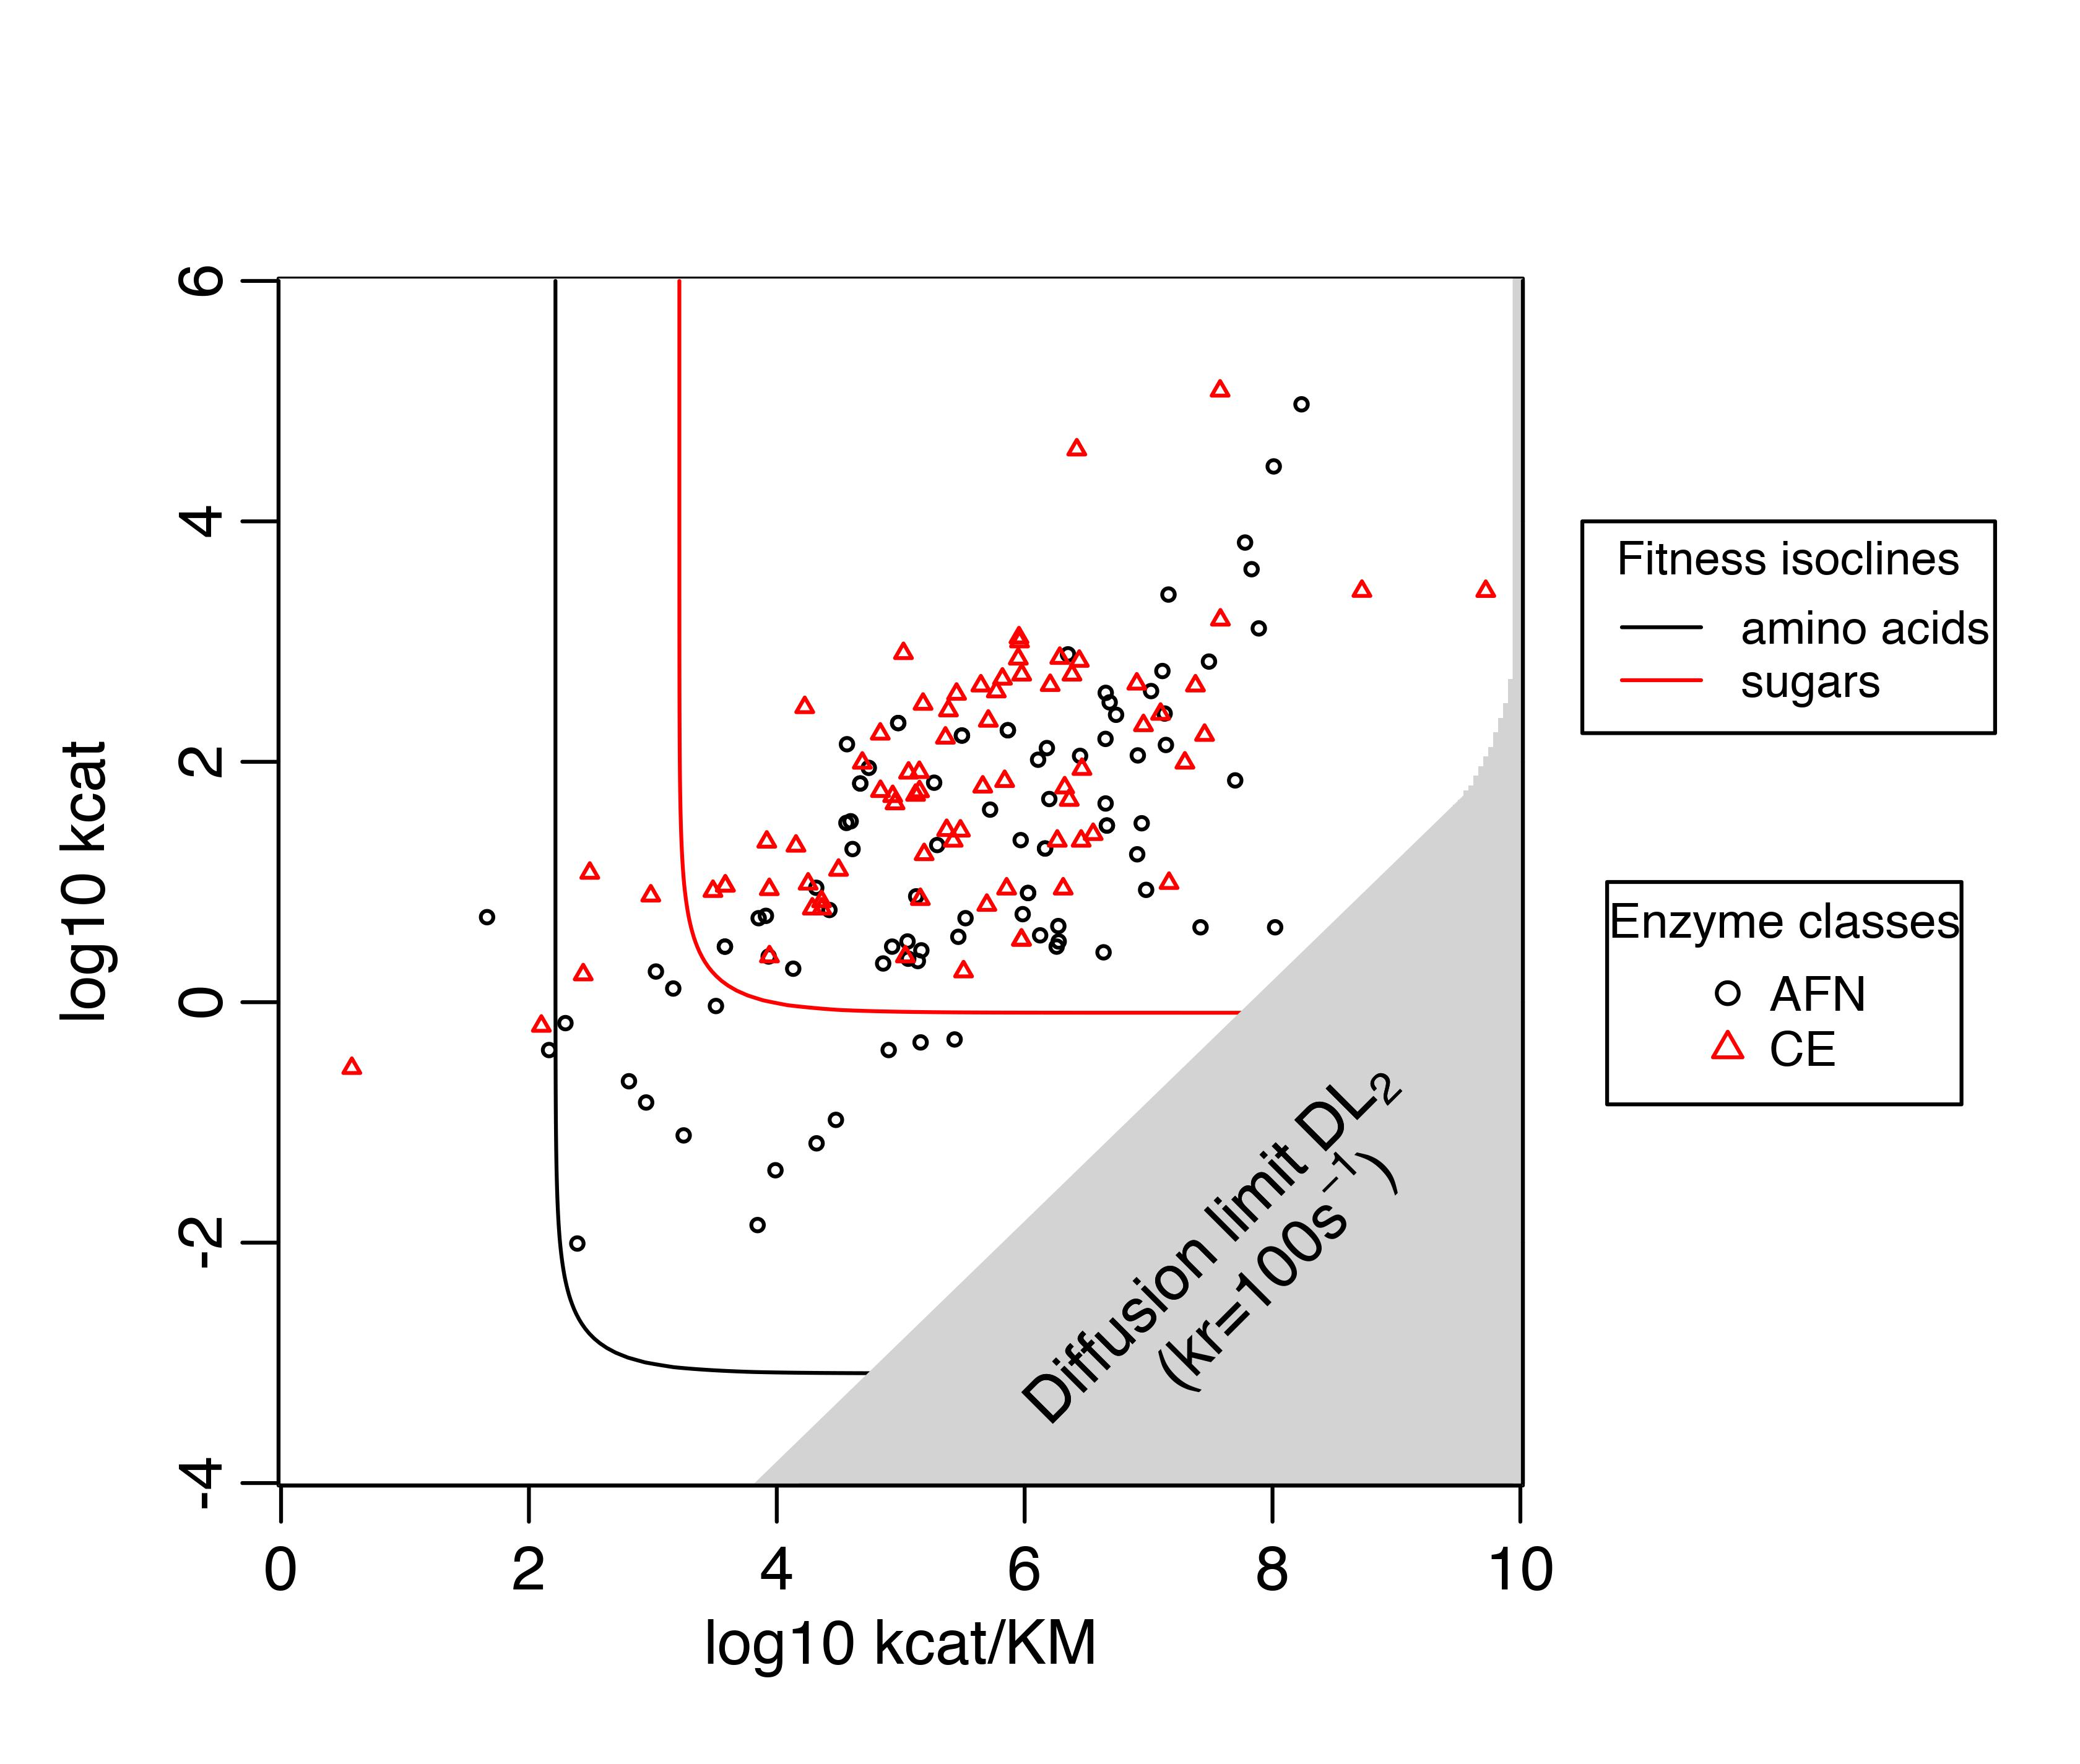
\includegraphics[scale=0.43,trim=0cm -0.75cm 0cm 1.5cm,clip]{Figures/2DFitContour_DataClasses.jpeg}  
\caption{\textit{in vitro} experimental estimates for enzyme kinetic parameters spread on the plateau of a generic theoretical fitness landscape. The parameter space considered corresponds to the usual empirical estimates for enzyme kinetic parameters $k_\text{cat}$ and $k{cat}/K_M$. The space is narrowed down here due to the diffusion limit, outlined by the grey area when $k_r$ is low ($10^2s^{-1}$), that impedes high values for $k_{cat}/K_M$ under low values for the ratio between $k_{cat}$ and $k_r$. In (A), the full dataset from \citep{Bar-Even11} is plotted in the parameter space and contrasted with the fitness landscape of the most upstream enzyme involved in amino acid or nucleoside metabolism (same parameters for transport than in Fig.~\ref{figure3D2DFit}, $[E_{tot}]=10^{-3}M$ and $k_r=10^{2}s^{-1}$). Most enzymes fall on the plateau of the fitness landscape. A few outliers overcome the diffusion limit, suggesting that $k_r$ might be lower than $10^2s^{-1}$ for these enzymes. In (B), the dataset is divided into classes identified by \citet{Bar-Even11}, with the acronym denoting enzymes involved in the central metabolism including (AFN): amino acids, fatty acids, and nucleotides  - and (CE): carbohydrates and energy. The isoclines shown correspond to parameter values typical of sugar transporters ($K_T=5mM$,$V_{Tm}=1mM.s^{-1}$) \citep{Maier02} or amino acids transporters (same as in (A)). With a few exceptions, enzymes seem to spread on the corresponding fitness plateau.}
\label{figure2D_BarEven_Dataset}
\end{figure*}

We then superimposed empirical estimates of kinetic parameters over our theoretical fitness landscapes, after substituting parameter $k_f$ for its usual empirical counterpart, $k_\text{cat} / K_M$. Because $k_{cat}/K_M \approx k_fk_{cat}/k_r$, this approximation only holds when $k_\text{cat} \gg k_r$. No less significantly, representing the fitness landscape in this parameter space
sets an area in the bottomright part of the landscapes where $k_f$ exceeds the diffusion limit (grey area on FIG.~\ref{figure2D_BarEven_Dataset}). For purposes of inclusiveness, we used $k_r=10^{2}s^{-1}$ by default -- noting that this limit would be displaced upwards for larger $k_r$ -- and otherwise used the same set of parameters as in FIG.~\ref{figure3D2DFit} to obtain FIG.~\ref{figure2D_BarEven_Dataset}. We see that a vast majority of the enzymes in the \citet{Bar-Even11} dataset belong to the fitness plateau. The implicit suggestion that this could be a result of Evolution on a common fitness landscape is surprising, as the dataset includes enzymes from many Eukaryote and Prokaryote species that contribute to various pathways. We instead anticipate that differences in evolutionary context should explain a part of the observed variance. We also note a strong linear positive relationship between $k_{cat}$ and $k_{cat}/K_M$ (\textbf{$R^2=0.4$}). This illustrates how focusing on $k_{cat}/K_M$ can be misleading if one's interest lies in mechanistic processes and their implications. Indeed, as obvious as it may sound, $k_{cat}$ and $k_{cat}/K_M$ are not independent from each other, especially when $k_\text{cat}<k_r$ (which is the case for a majority of the data points in FIG. \ref{figure2D_BarEven_Dataset}). Concluding on whether a positive relationship between $k_f$ and $k_\text{cat}$ does exist would require to estimate $k_r$ for each enzyme.

Because we have previously shown that different transporters may yield plateaus with different shapes (\textit{e.g.} for sugars and amino acids), our model predicts that enzymes involved in the corresponding pathways should have their own specific distributions. Representing findings by  \citep{Bar-Even11} suggests that there may indeed be an explainable difference between enzymes contributing to carbohydrate processing (in red in FIG.~\ref{figure2D_BarEven_Dataset}-B) and to that of amino acids (a part of the black dots in FIG.~\ref{figure2D_BarEven_Dataset}-B). %But, as we shall nevertheless emphasise, a proper analysis should include many other variables that may also contribute to the variance between enzymes.
This apparent discrepancy in fitness landscapes across pathways starting with different transporters can only explain a small part of the wide distribution of kinetic parameters reported by \citet{Bar-Even11}, thus requiring a careful study of other evolutionary, ecological and chemical parameters.

\subsection{Evolutionary dynamics of enzyme kinetic parameters}

\begin{figure*}[h!]
\centering
\begin{minipage}[c]{0.48\linewidth}
\includegraphics[scale=0.64,trim=0cm 0cm 3cm 1.5cm,clip]{Figures/2DFitLandscape_Evo_Results_lowF_nobias.jpeg}
\end{minipage} \hspace{-0.5cm}%\hfill
\begin{minipage}[c]{0.48\linewidth}
\includegraphics[scale=0.64,trim=1cm 0cm 0.5cm 1.5cm,clip]{Figures/2DFitLandscape_Evo_Results_lowF_withbias.jpeg} 
\end{minipage}
\caption{Simulations of a population genetics model indicate that enzymes should spread on a plateau corresponding to their effective population size $N_e$ only when mutations are unbiased; mutations biases towards lower efficiencies make enzymes stick to isoclines, such that their evolution is predictable. The case considered here is that of a transporter with a low flux at saturation and high affinity ($V_{Tm}=1\mu Ms^{-1}$ and $K_T=10\mu M$) -- under various scenarios: four effective population sizes from $10^2$ to $10^5$ (different colors) and three cases of mutational biases(($b=0$ corresponds to the absence of mutational bias). We ran 30 independent simulations for each scenario, each represented a dot in the ``empirical" parameter space ($k_\text{cat}, \;k_\text{cat}/K_M$). Only $k_\text{cat}$ and $k_f$ were susceptible to evolve, while $k_r$ was set to $10^3s^{-1}$ such that the grey part of the parameter space is inaccessible to enzymes due to the diffusion limit. At evolutionary equilibrium, enzyme efficiencies reach a plateau delineated by an isocline indicative of effective selection. In (A), no mutational bias results in enzymes spreading onto the plateau, some reaching very high $k_\text{cat}$ and/or $k_\text{cat}/K_M$ values, while in (B) enzyme efficiencies stick to their predicted isoclines -- under the Nearly Neutral Theory of Evolution \citep{Ohta92} -- owing to the over-representation of mutations reducing enzyme efficiencies.% The stickiness is self-evidently correlated to the average mutational bias $b$.
}
\label{figure2D_Evolutionary_results}
\end{figure*}

To approach how populations evolve on the fitness landscapes drawn through our mathematical model, we built a simple population genetics model that includes, besides selection, mutation and drift. In this individual based model, absolute fitness is directly proportional to the flux of product at equilibrium -- which itself equals the inward flux of nutrients. We consider the flux of the first enzyme (see Methods and previous Results sections for details), as presumably the evolutionary dynamics should be similar for downstream enzymes with similar landscapes. Two different levels of metabolic demands were considered, corresponding to parameter values used to draw panels (A) and (I) in FIG.~\ref{figure2DSEns} in order to control that differences in the delineation of the plateau (in the parameter space) do not affect the evolutionary equilibrium. For the enzyme of a given individual, only $k_\text{cat}$ and $k_f$ were susceptible to evolve through mutations. Mutational effects on $\log_{10}k_{cat}$ and $\log_{10}k_f$ were drawn from independent normal distributions with mean $b \leq 0$, with the absolute value of $b$ setting the intensity of mutational towards less efficient parameter values. The standard deviation of the distribution of mutational effects was set to $0.3$ such that most mutations explore the neighbouring parameter space, with rare mutations allowing changes by more than one order of magnitude (one $\log_{10}$ unit) at a time, accordingly to values reported in \citep{Carlin16}. %Simulations were performed for Ne ranging from $10^2$ to $10^5$ individuals, and replicated 30 times for each set of parameter. (en matériel et méthodes, de toute façon on le voit avec les résultats)


\begin{figure*}[h!]
\centering
\begin{minipage}[c]{0.48\linewidth}
\hspace{-1.3cm}
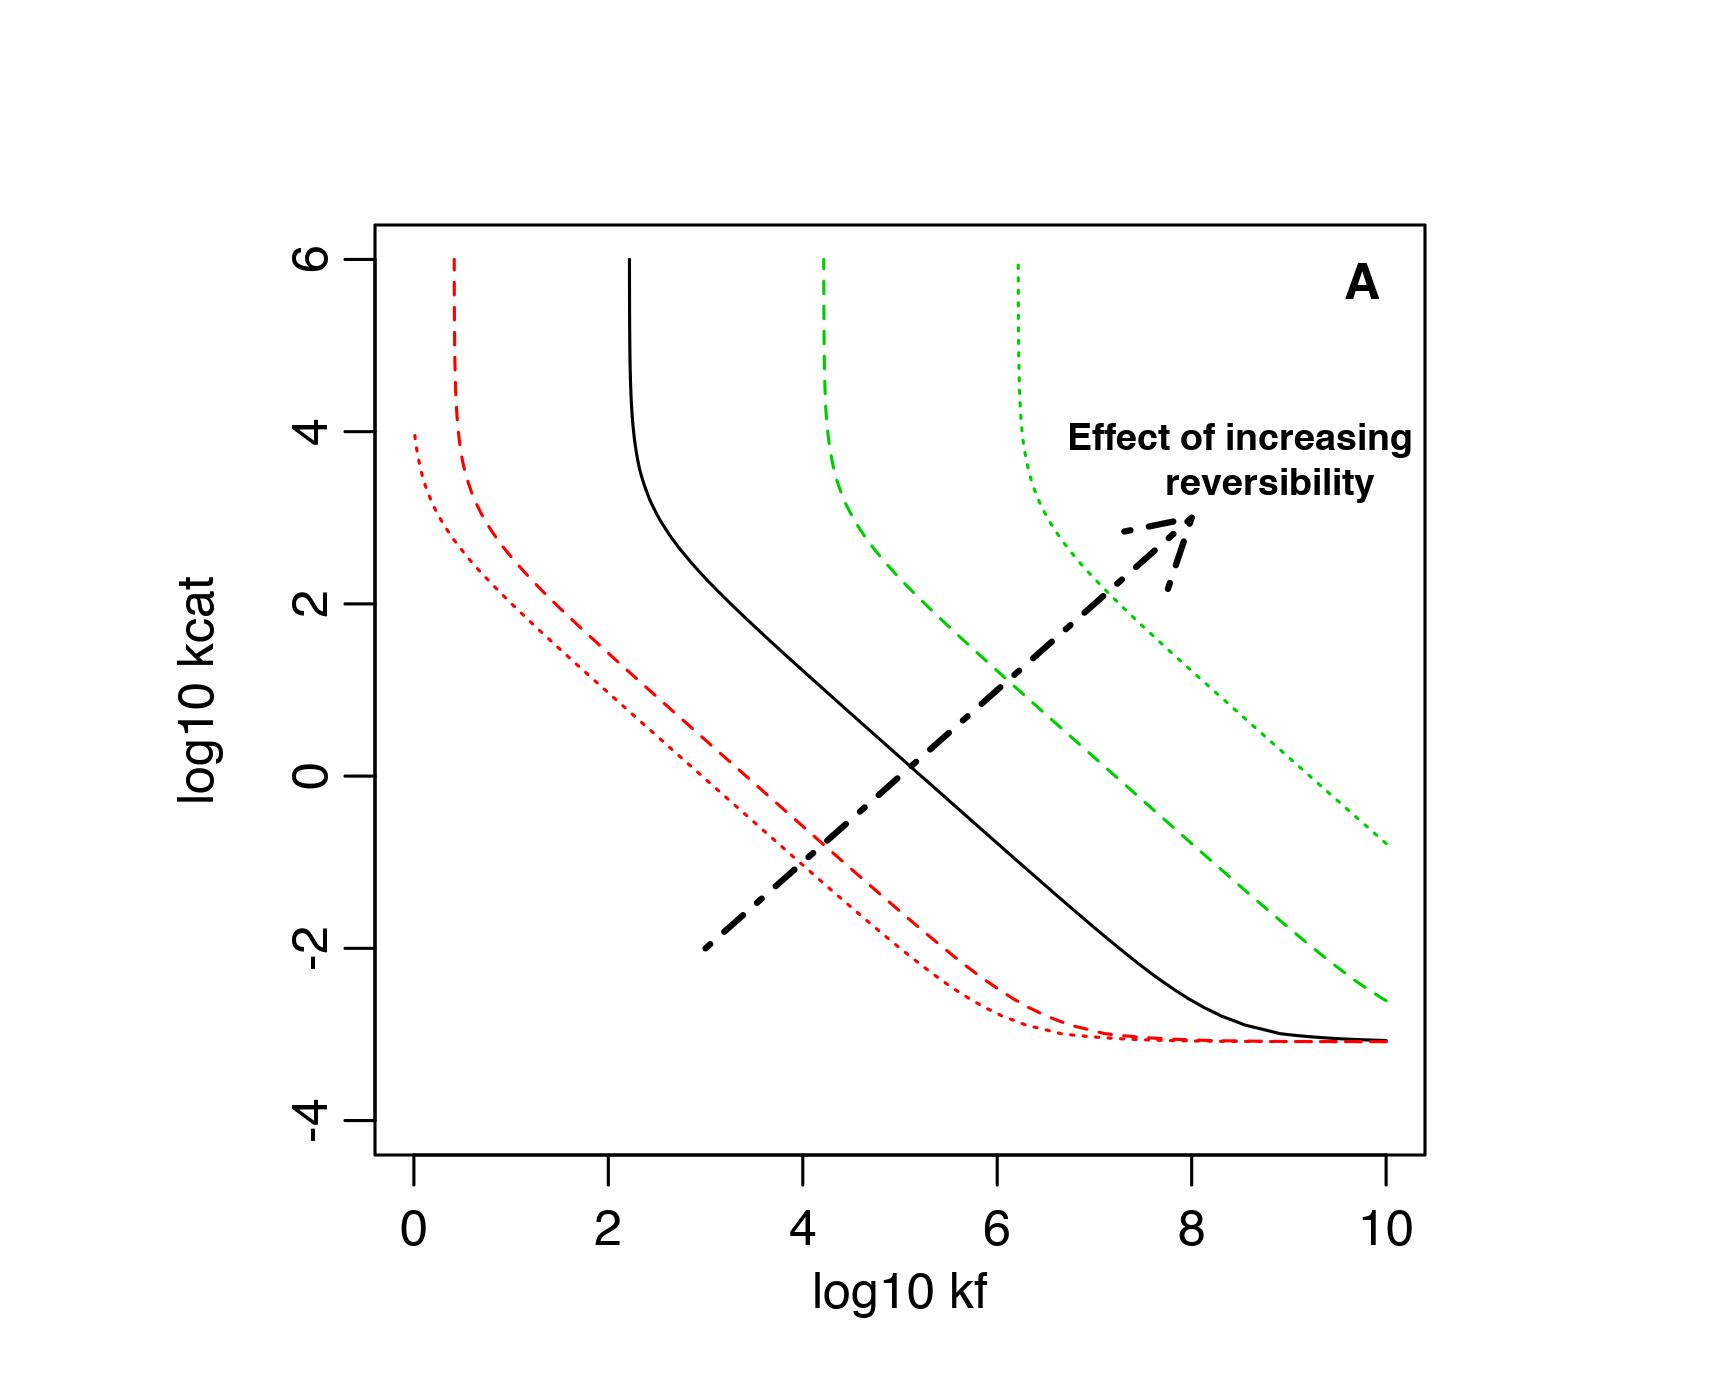
\includegraphics[scale=0.64,trim=0cm 0cm 0cm 1.5cm,clip]{Figures/2DFitLandscape_Multiple_Reverse.jpeg} 
\end{minipage} \hspace{-1.3cm}
\begin{minipage}[c]{0.48\linewidth}
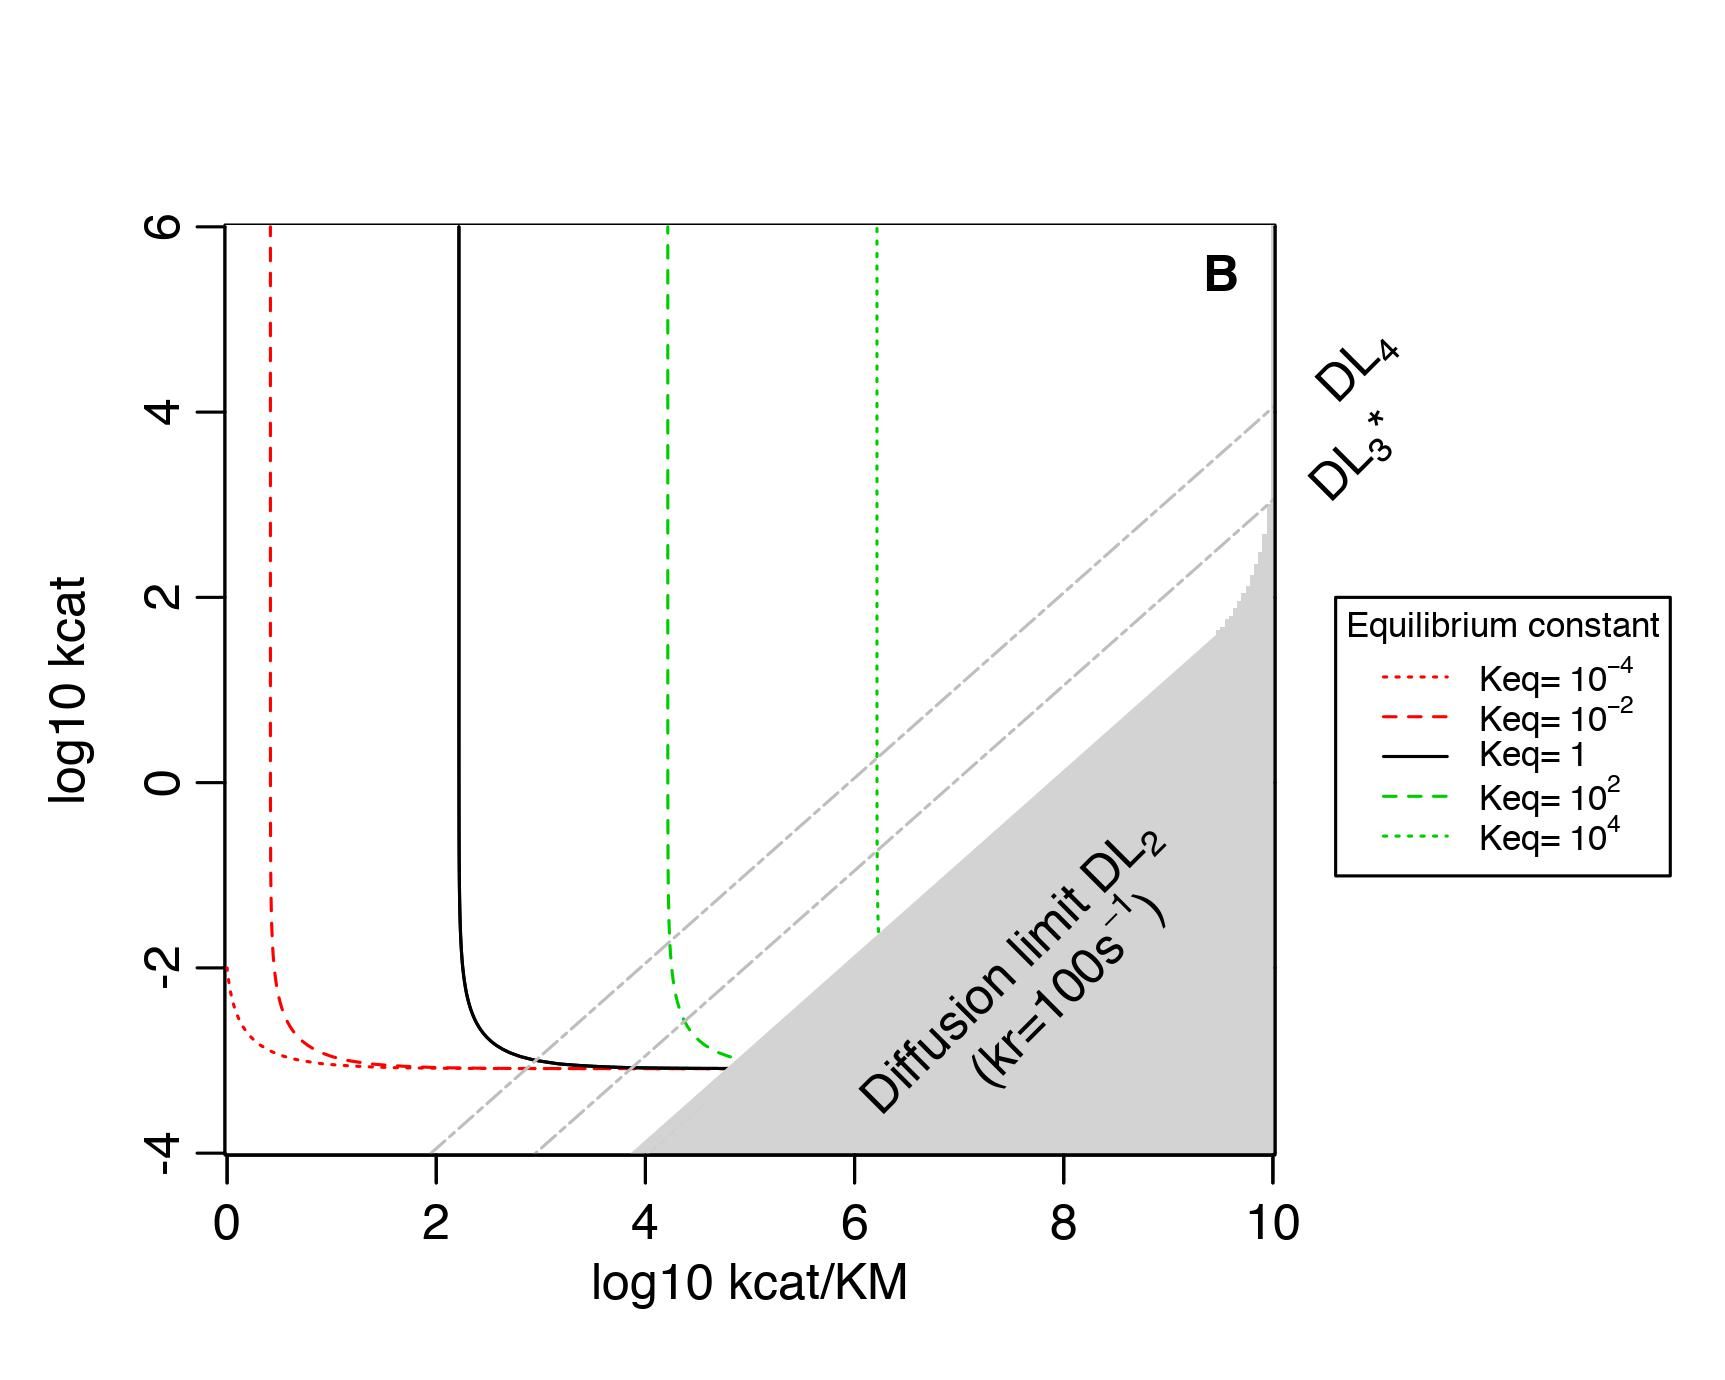
\includegraphics[scale=0.64,trim=0cm 0cm 0cm 1.5cm,clip]{Figures/2DFitLandscape_Multiple_Reverse_exp_par.jpeg}
\end{minipage}
\caption{Backwards reaction rates of an enzyme directly upstream have a strong impact on the fitness landscape. Both plots show results of the influence of the reversibility of the first reaction on the fitness landscape of the next enzyme. Parameters are identical as in FIG.~\ref{figure3D2DFit}, corresponding to the model case for amino acids, with $k_r=10^3s^{-1}$. $K_{eq}$ equals $[S]_{eq}/[P]_{eq}=k_rk_{inh}/k_\text{cat}k_f$ \citep{Klipp94} and quantifies the degree of reversibility, a low $K_{eq}$ featuring low reversibility and vice versa. The first enzyme is a nearly perfect forward enzyme with $k_f=10^{8}M^{-1}$ and $k_{cat}=10^4s^{-1}$. 
Reversibility was equally spread between the two backwards parameters (\textit{e.g.} $K_{eq}=10^2$ yields $k_r=10^{1}k_{cat}$ and $k_{inh}=10^{1}k_f$), and a low degradation rate was considered ($\eta_d=10^{-4}s^{-1}$). In (A), results are plotted in the theoretical parameter space ($k_f, \; k_\text{cat}$), showing that any increase in reversibility increases the pressure on enzyme kinetics by the same magnitude -- except when reactions are highly non-reversible (in red)
. In (B), the same results are shown in the experimenter parameter space of the second enzyme, showing that there is an increased pressure on $k_\text{cat}/K_M$ under higher reversibility. 
While the plateau is not moved upwards, indicative of a selection on $k_\text{cat}$ independent on reversibility when $k_\text{cat}/K_M$ is fixed, positive selection for this parameter may still arise due to the diffusion limit that precludes the access to the lowest $k_\text{cat}$ at high $k_\text{cat}/K_M$. The diffusion limit should play an important role for enzymes with a high dissociation rate $k_r$, as illustrated by the delineation of the diffusion limit (grey area or grey dashed lines) corresponding to several $k_r$ values (eg. DL$_3$ stands for $k_r=10^3s^{-1}$; the star indicates that it is the case represented in (A)).}
\label{figure2D_Reverse}
\end{figure*}

Without any mutational bias ($b=0$), simulated enzymes spread all over the fitness plateau, as expected (FIG.~\ref{figure2D_Evolutionary_results}A for low flux, Figure S7A of SM otherwise). The onset of the plateau depends on the strength of drift and hence derive from the effective population size $N_e$, following the classical expectation that selection becomes inefficient when $N_e \times s < 1$ \citep{Kimura68}. Introducing a mutational bias that makes enzyme kinetics less efficient on average has a strong effect on both $k_\text{cat}$ and $k_f$, preventing simulated enzymes from improving far above the drift barrier (FIG.~\ref{figure2D_Evolutionary_results}B for low flux, Figure S7B of SM otherwise).
Even weak biases ($b=0.1$) lead to enzymes evolving in the vicinity of the isocline where $N_e \times s \approx 1$. Increasing the strength of this bias to $0.2$ only slightly decreases the population variance around this expectation.

In light of this effect of the effective population size on enzyme evolution, the seeming adequation between the plateau and the data in FIG.~\ref{figure2D_BarEven_Dataset} appears puzzling, as the lowest $N_e$ considered here do not encompass those traditionally found for unicellular organisms that mostly exceed $10^5$ \citep{Bobay18}.
In the same vein, Eukaryotes and Prokaryotes datasets display similar ranges despite large differences in effective population sizes \citep{Bar-Even11}. It is thus possible that the role of genetic drift is not well captured by a model that considers small parts of a large system in isolation, or more generally that the link between fitness and flux is not as straightforward as we have assumed. Notwithstanding this issue, the prediction of enzymes evolving a predictable set of kinetics parameters when mutational biases are considered contrasts with the broad variability reported \citep{Davidi18}, thereupon requiring further investigation.

\subsection{Explaining the variance within a pathway}

So far, our model predicts that enzymes intervening in a given pathway should evolve on a common fitness landscape, provided that the accumulation of intermediate metabolites is highly detrimental. This should produce similar enzymes along a pathway, which is directly contradicted by empirical estimates, suggesting that each enzyme instead evolves on its own fitness landscape. In this section we show that (1) physical constraints, among which in first place is the reversibility of reactions and (2) the joint evolution of kinetic parameters and other evolving parameters, can explain large differences among enzyme kinetic parameters by influencing actual \textit{in vivo} efficiencies. %evolvable=susceptible to adapt by NS, peut-être qu'on veut être plus général, mutable?

Reversibility is an intrinsic feature of chemical reactions that cannot be directly overcome by Evolution \citep{Haldane30,Cornish-Bowden79a}. A highly reversible reaction corresponds to a large intrinsic equilibrium constant $K_{eq}=[S]_{eq}/[P]_{eq}$ \citep{Klipp94}, and results in higher backward than forward rates in the following chemical equation: \begin{equation}
\ce{ E + S <=>[k_{f}][k_{r}] ES <=>[k_{cat}][k_{inh}] E + P_1 },
\label{chemMM_fullrev}
\end{equation}
where $k_{inh}$ represents the rate at which enzyme and product combine back. Such a (reversible) reaction could in principle influence the selective pressure acting on the following enzyme in the pathway, for both enzymes compete to process the same metabolite $P_1$. We thus quantified how reversibility affects the evolution of an enzyme downstream (FIG.~\ref{figure2D_Reverse} ; using the same model case parameters used throughout the paper (see FIG.~\ref{figure3D2DFit}
for details) and considering a nearly perfect first enzyme for consistency: $k_{cat}=10^4s^{-1}$,$k_f=10^8M^{-1}s^{-1}$).

The equilibrium constant $K_{eq}$ has a similar (non-linear) impact on the fitness landscape of the second enzyme than the degradation rate, with a highly reversible upstream enzyme exerting a selection pressure downstream towards an increase of kinetic parameters (FIG.~\ref{figure2D_Reverse}-A). Indeed, increasing $K_{eq}$ moves the fitness plateau toward the upper-right corner in the ($k_f$,$k_\text{cat}$) parameter space, hence selecting for more efficient downstream enzymes. The effect appears linear, except for very low values of $K_{eq}$ where it fades -- such that a 100-fold change in $K_{eq}$ has little impact -- because the main issue when reactions are highly non-reversible becomes, again, metabolite accumulation. Therefore, the reversibility of the upstream reaction appears like a critical parameter for the evolution of an enzyme, able to generate large changes in evolutionarily expected kinetic parameters. When using the ``empirical" parameter space (FIG.~\ref{figure2D_Reverse}-B), we observe that increasing reversibility only selects for higher $k_\text{cat}/K_M$. Interestingly, the unbinding rate $k_r$ of an enzyme, which is correlated to its reversibility, may eventually favour a positive codependency between the forward rates $k_\text{cat}$ and $k_f$ as the latter is no longer sufficient to ensure a high $k_\text{cat}/K_M$ (see FIG.~\ref{figure2D_Reverse}-B and Figure S9 of SM for this influence in the theoretical parameter space).

\begin{figure}[t!]
\centering
\includegraphics[scale=0.58,trim=0cm 0cm 0cm 1.5cm,clip]{Figures/Plot2DFitLandscape_Enz_conc.jpeg} 
\vspace{-0.3cm}
\caption{High enzyme concentration $[E_{tot}]$ alleviate selection on both $k_\text{cat}/K_M$ and $k_\text{cat}$. The parameters for transport are the same than in FIG.~\ref{figure3D2DFit}, with $k_r=10^3s^{-1}$.}
\label{figure2DEnzconc}
\end{figure}

Hitherto, we have considered enzymes to be highly concentrated, an assumption that we relax here. Predictably, increasing the concentration of the first or second enzyme in a pathway releases the selection on their kinetic parameters \citep{Noor16}, producing larger fitness plateaus as an enzyme concentration increases (see FIG.~\ref{figure2DEnzconc} for the first enzyme and Figure S10 of SM for the second). Because the concentration is subject to heritable changes \citep{Schaefke13}, we anticipate that the joint evolutionary dynamics of the concentration and kinetic parameters should yield a negative correlation between them, as reported by \citet{Davidi16,Davidi18} (who focused on $k_\text{cat}[E]_{tot}$), due to the compensatory effect of concentration.

\section{Discussion\label{sec:Discussion}}

Most enzymes have been considered to be only moderately efficient, if not sloppy \citep{Bar-Even11,Bar-Even15}. This claim was put into perspective by \citet{Newton18} who argued that the link between fitness and enzyme efficiencies is complex and may be partly enzyme-dependent. Through this work, we have developed a model where enzyme efficiencies are mechanistically linked to fitness through the impact of nutrient gradients on the production of metabolites. Our results emphasize that enzymes might in fact be quite efficient and, possibly, as efficient as Evolution allows. 

We have modelled two processes of nutrient uptake that rely heavily on concentration gradients: passive (PD) and facilitated diffusion (FD). Our results apply to the numerous metabolic pathways that start with them, and also possibly to the widely used secondary active transport (SAT) in which FD of ion-substrate complexes follows the active extraction of a cotransported ion. Indeed, SAT can be described by similar equations as FD, with the difference that energy is required for extraction \citep{Stein86e}.

Our results indicate that an enzyme's forward kinetic parameters -- $k_\text{cat}$ and $k_f$ -- evolve on cliff-like fitness landscapes with a plateau -- where the flux of energy generated increases on a log scale -- surrounded by a steep slope. This conclusion seems to agree qualitatively with the assumptions of previous models \citep{Hartl85,Kaltenbach14}, which we confirm here from a nutrient driven perspective.
Importantly, our framework allows to consider the joint evolution of two kinetic parameters, $k_f$ and $k_\text{cat}$ instead of a composite ``efficiency" whose relevance is questionable \citep{Koshland02,Eisenthal07}, and to pinpoint model parameters that have a differential impact on each. This, along with our broad comparison of model predictions with a massive dataset, initiates an attempt to predict evolutionary trends at the level of individual enzymes. We show that this should be possible in principle, under the assumption that mutations of efficient enzymes are slightly biased towards making them less efficient, which limits evolutionary predictions to a narrow range in the parameter space.

Overall, the evolution of an enzyme should result from an interplay between (1) ecological and biochemical factors -- metabolic demands, richness of the environment, reversibility of reactions -- that draw the landscape, and (2) evolutionary factors -- effective population size, distribution of mutational effects -- governing how organisms move through evolutionary times on these landscapes. We have effectively found that the shape of the fitness landscape depends on features of the transporter, namely the maximum flux they can sustain and their affinity for the substrate, each having different effects on $k_\text{cat}$ and $k_f$. These features are themselves evolving quantities, and the joint evolution of transporters and intracellular enzymes remains to be studied. Yet, using parameters that correspond to empirical estimates for sugars and amino acids, we have found that enzymes intervening in subsequent metabolic pathways should be different, with those in the ``sugars" pathway being selected for faster kinetics. The focus in this study was not on interactions within a pathway and high-order epistasis, but our framework suggests that all enzymes but the first in a pathway should evolve on fitness landscapes that do not depend on their position, as long as all upstream enzymes belong to the fitness plateau. If one enzyme is noticeably inefficient, however, selection will push downstream enzymes towards a wider plateau, as a larger region of the parameter space can accommodate such a lower flux.

We also notice that different constraints may be met along a pathway and make each enzyme evolve on its own fitness landscape, possibly explaining a part of the large variance reported at this scale. Physical constraints may for instance act differentially on different enzymes, as exemplified by the intrinsic reversibility of a reaction that fuels the selective pressure towards higher efficiency in downstream enzymes. This may contribute to explain the high efficiency of a few specific enzymes, and thereby why there exists some ``equilibrium enzymes" pushing reactions close to equilibrium \citep{Williamson67,Davidi18}.
Aside from physical constraints, actual enzyme kinetic parameters are entangled with many more biochemical parameters, making the prediction of their evolution complex. 

More specifically, we have examined the effect of one such parameter (but not its evolution), the concentration of the enzyme, showing that it indeed exerts an important role and is likely involved in the variance in $k_f$ and $k_\text{cat}$, for low efficiency can be buffered by high levels of expression and vice versa. How enzyme levels of expression and efficiencies jointly evolve, including the role of the cellular content on these efficiencies, should be the next step forward in the understanding of enzyme evolution. Because a cell is packed with many organites and biomolecules, making diffusion less efficient and $k_f$s lower \textit{in vivo} than their \textit{in vitro} counterparts, opposing forces govern the evolution of enzyme concentrations. Increasing concentrations may thus come at a great cost by slightly but steadily decreasing the actual efficiency of many catalysts at once, in turn favouring the evolution of highly efficient enzymes unless physical constraints prevent such an improvement.

Our work provides a mechanistic model for enzyme evolution, based on the assumption that enzymatic efficiency helps ingesting nutrients and win the competition for resources. Unfortunately, mechanistic does not mean free of a definition of fitness, as we have assumed that the latter is proportional to metabolic flux, hence considering each flux in isolation. Fitness instead results from a wide range of metabolic pathways that combine together and should all be competitive to certain degrees. How high-order epistasis builds up, and genetic drift acts in this context, is far from obvious; but this should not impact much how enzymes evolve in old, overall efficient pathways, as any impediment in efficiency should have an independent effect on fitness in this context, as captured by our model. Yet, this could make selection weaker in some or all pathways, as exemplified by \citet{Heckmann18}, and therefore help explain why they appear to be evolutionary suboptimal. But more importantly, such a model would be crucial to understand how metabolic pathways arose and improved, likely from a highly inefficient state during early steps in the evolution of life on Earth.

\section{Materials and Methods\label{sec:M&M}}

\subsection{Quantifying the maximum size for cells using passive diffusion}

If a cell is to be viable, it has, at least, to uptake enough glucose to compensate for basal metabolism -- metabolism that allows to maintain the same cell size for non-actively growing cells \citep{Lynch15} -- leading to the following equation: $\phi_{PD}=C_M$, with $\phi_{PD}$ the uptake through passive diffusion and $C_M$ the basal metabolism demand. To calculate the maximum size a cell can reach using only passive diffusion, we relied on the formula $C_M=0.39V^{0.88} (10^9 ATP/hr)$ estimated in \citep{Lynch15}. We also assumed the cell to be of spherical shape, both concentrations -- inside and outside the cell -- to be constant with the cellular concentration staying so low that it can be overlooked, meaning that the uptake resulting from passive diffusion can merely be written as $\phi_{PD}=P.[S_{\text{out}}].\frac{SA_{\text{sphere}}}{V_{\text{sphere}}}$, where $SA_{\text{sphere}}$ and $V_{\text{sphere}}$ are the surface area and the volume of a sphere, and $P$ represents the cell permeability and was measured to $10^{-6}\mu m^{-1}$ \citep{Wood68} for glucose. Finally, we considered that each glucose yields 30 ATP molecules \citep{Rich03}. 

\subsection{Flux sustained by the first enzyme}

When assessing the flux of product made by the first enzyme in a pathway, both (PD) and (FD) result in similar sets of equations; we focus on FD here (see Text S5 - Mathematical appendix in Supplementary material for a comparison with PD). FD typically relies on the specific binding of substrate molecules -- located outside the cell -- by transmembrane carrier proteins, followed by their translocation into the cytoplasm \citep{danielli1954,Wilbrandt61,Kotyk67}. This specific process obeys Michaelis Menten-like kinetics when transport is assumed to be symmetric \citep{Kotyk67}, which can be modelled through Briggs-Haldane equations \citep{Briggs25,Haldane30,Stein86d}:
\small
\begin{equation}
\frac{d[S_\text{in}]}{dt}=V_{Tm}.\frac{[S_\text{out}]-[S_\text{in}]}{K_T+([S_\text{out}]+[S_\text{in}])+\alpha.\frac{[S_\text{out}][S_\text{in}]}{K_T}}
\end{equation}
\normalsize

with:
\small
\begin{equation*}
  \left\{
      \begin{aligned}
		&V_{Tm}\text{: the maximum rate of a given carrier protein;}\\
		&K_T\text{: a constant inversely proportional to the transpor-}\\
		&\text{  ter efficiency};\\
		&\alpha \text{ : the Kotyk interactive constant  capturing the dis-}\\
		&\text{  equilibrium between bound and free transporters.}
      \end{aligned}
    \right.
\end{equation*}
\normalsize

%Alongside the concentration gradient, the Kotyk interactive constant \cite{Kotyk67} also brings by something special because the efflux (\textit{i.e. outwards flow}) cannot be overlooked due to the emergence of saturation in the process \citep{Teusink98,Bosdriesz18}.
By construction, $\alpha$ cannot exceed 1 \cite{Kotyk67} and is close to this upper limit for sugars (\textit{e.g.} $\alpha=0.91$ for glucose \citep{Teusink98}, so we set $\alpha=1$ by default in this study, maximizing the effect of interaction).

A model including both FD and irreversible substrate conversion by an enzyme therefore corresponds to the following chemical equation:

\begin{equation}
\footnotesize
\schemestart
 S$_{out}$
 \arrow{<=>[$V_{Tm},K_T$][$\alpha$]}
 S$_{in}$ + E
 \arrow{<=>[$k_{f}$][$k_{r}$]}
 ES
 \arrow{->[*0$k_{\text{cat}}$]}
 E + P$$
\schemestop
\label{chemMMT1R}
\end{equation}

Using analytical tools (see \citet{Kuile94}, rederived in Supplementary material - Text S5 Mathematical appendix), the flux can be determined through the following set of equations:

\vspace{-0.25cm}
\small
\begin{align}
\strut
[ES]^*=\frac{k_f[S_{in}]^*}{k_{r}+k_{cat}+k_f[S_\text{in}]^*}.[E_{tot}]\\
v=\frac{d[P]}{dt}=k_{cat}[ES]^*
\end{align}
\normalsize

where:
\vspace{-0.25cm}
\small
\begin{align}
[S_\text{in}]^*=\frac{-b+\sqrt{b^2-4ac}}{2a}
\end{align}
\normalsize

with:
\small
\begin{equation}
  \left\{
      \begin{aligned}
        a&=k_f k_{cat}[E_{tot}](1+\frac{[S_{in}]}{K_T})+k_fV_{Tm}\\
		b&=k_f k_{cat}[E_{tot}]([S_{in}]+K_T)+(k_{cat}+k_r-k_f[S_{in}])V_{Tm}\\
		c&=-V_{Tm}[S_{in}](k_r+k_{cat})\\
      \end{aligned}
    \right.
\end{equation}
\normalsize

%\vspace{-0.5CM}
% Because of the Kotyk interaction constant -- set to $1$ -- the flux cannot reach the value of $V_{Tm}$, and rather stabilizes around an amount of product formed $\frac{d[P]}{dt}=0.9\mu M.s^{-1}$. In SM possibly

\subsection{Multiple enzymes model}

In order to study the evolution of downstream enzymes, we considered an unbranched metabolic pathway in which the product formed by the first reaction serves as the substrate for a second reaction. Theoretically, as there is nothing prohibiting increase in product concentrations -- for it is not considered reversible at this point -- any second enzyme should be able to sustain any metabolic demand. We penalized large increases in cellular concentrations through a degradation process of the product of the first reaction, occurring at rate $\eta_d$ ($\times$ this concentration). Under these new assumptions, the chemical reactions occurring after uptake (Michaelis Menten part of Eq.\ref{chemMMT1R}) are described by the following equations:

\small
\begin{align}
\schemestart
 S$_{in}$ + E$_1$
 \arrow{<=>[$k_{f1}$][$k_{r1}$]}
 E$_1S$
 \arrow{->[*0$k_{\text{cat}1}$]}[0]
 E$_1$ + P$_{1}$
 \schemestop
 \label{chemMMT1R_deg}
 \end{align}
 \begin{align}
 \schemestart
 P$_{1}$ + E$_2$
 \arrow{<=>[$k_{f2}$][$k_{r2}$]}
 E$_2$P$_1$
 \arrow{->[*0$k_{\text{cat2}}$]}[0]
 E$_2$ + P$_{2}$
 \arrow(@c1--){->[*0$\eta_d$]}[-90]
 P$_{1out}$
\schemestop
\label{chemMMT2R_deg}
\end{align}
\normalsize

Such a system may reach a steady-state at which the cellular concentrations of the substrate $S_{in}$ and of the first product $P_1$ are constant. At this point, the net instantaneous uptake of substrate (through the membrane) equals the instantaneous production of $P_1$ which, in turn, equals the addition of the instaneous amount of degraded $P_1$ and the instantaneous production of $P_2$, according to the principle of mass conservation. It yields the following system of equations:

\footnotesize

\begin{equation}
		\begin{aligned}
V_{Tm}.&\frac{([S_{out}]-[S_{in}])}{K_T+([S_\text{out}]+[S_\text{in}])+\alpha.\frac{[S_\text{out}][S_\text{in}]}{K_T}}=V_{m1}.\frac{[S_{in}]}{K_{M1}+[S_{in}]}
		\end{aligned}
		\label{mathMMT1R_deg}
\end{equation}

\begin{equation}
\begin{aligned}
V_{m1}.&\frac{[S_{in}]}{K_{M1}+[S_{in}]}=V_{m2}.\frac{[P_1]}{K_{M2}+[P_1]}+\eta_d.[P_1]
		\end{aligned}
		\label{mathMMT2R_deg}
\end{equation}
\normalsize
\noindent where appear the traditional Michaelis-Menten kinetic parameters for the (i$^{eth}$) reaction:
\small
\begin{equation*}
  \left\{
      \begin{aligned}
		&V_{m_i}=k_{cat_i}[E_{tot_i}]\\
		&K_{M_i}=\frac{k_{r_i}+k_{cat_{i}}}{k_{f_{i}}}
      \end{aligned}
    \right.
\end{equation*}
\normalsize

In an independent section, we also introduced reversibility to further the analysis, through the modification of equation \ref{chemMMT1R_deg}, which becomes:

\begin{align}
\small
\schemestart
 S$_{in}$ + E$_1$
 \arrow{<=>[$k_{f1}$][$k_{r1}$]}
 E$_1S$
 \arrow{<=>[*0$k_{\text{cat}1}$][$k_{inh1}$]}[0]
 E$_1$ + P$_{1}$
 \schemestop
 \label{chemMMT1R_degrev}
 \normalsize
 \end{align}
 
Such a phenomenon is described by the more general form of Haldane equation \citep{Haldane30,Cornish-Bowden79a}, which changes the contribution of the first reaction ($V_{m1}.\frac{[S_{in}]}{K_{M1}+[S_{in}]}$) in both equations (\ref{mathMMT1R_deg}) and (\ref{mathMMT2R_deg}) to:
\footnotesize
\begin{equation*}
		\begin{aligned}
		V_{m1^{+}}.&\frac{[S_{in}]}{K_{M1^{+}}+[S_{in}]+K_I [P_1]}-V_{m1^{-}}.&\frac{[P_1]}{K_{M1^{-}}+[P_1]+[S_{in}]/K_I}
		\end{aligned}
		\label{mathMMT1R_rev}
\end{equation*}
\normalsize
with $V_{m1^{+}}$ and $K_{M1^{+}}$ respectively correponding to the previous $V_{m1}$ and $K_{M1}$, while:
\small
\begin{equation*}
  \left\{
      \begin{aligned}
		&V_{m1^{-}}=k_{r1}[E_{tot1}]\\
		&K_I=k_{inh1}/k_{f1}\\
		&K_{M1^{-}}=K_{M1^{+}}/K_I
      \end{aligned}
    \right.
\end{equation*}
\normalsize

To solve these systems, which are not easily tractable analytically -- for they rely on cubic equations -- we implemented the Newton method \citep{Atkinson89} aiming to find $[S_{in}]^*$ and $[P_1]^*$. We ran the algorithm starting from very low values of concentration (both set to $10^{-20}M$) to determine numerically the equilibrium without facing convergence problems. The final flux can then be determined through the ``production'' part of equation (\ref{mathMMT2R_deg}), \textit{i.e.} $V_{m2}.\frac{[P_1]}{K_{M2}+[P_1]}$.

\subsection{Validation of the method and computing of the fitness landscapes}

To validate the approach, we compared equilibrium results obtained with Raphson-Newton algorithm to those obtained when simulating the process with Euler explicit schemes for a set of (3x3) kinetic values -- $k_\text{cat}$ and $k_f$ -- encompassing three orders of magnitude (see SM - Section Text 5 for further details).

In each section, we then determined the flux achieved for enzyme kinetic parameters $k_\text{cat}$ and $k_f$ varying by 10 orders of magnitude, setting $k_r$ to $10^3 s^{-1}$ -- within the range found for several enzymes \citep{Klipp94,Knowles77} -- unless stated otherwise. Except in the section dedicated to the influence of enzyme concentration, we set the enzyme concentration such that $[E_{tot}]=1mM$, lying nearby the highest observed values \citep{Albe90,Noor16}. Other parameters are detailed on a case-by-case basis as they may change depending on the goal of each section. To compare with the data and visualize results in the experimenter's parameter space, we also determined the flux and plotted simulation results using $k_\text{cat}$ and $\frac{k_\text{cat}}{K_M}$, also making them vary by 10 orders of magnitude. Fitness was considered to be linearly related to the flux in a pathway. To compute fitness landscapes, we thus divided the parameter space in 100 equidistant values on a log-scale (250 for representations with $k_{cat}/K_M$ to draw a cleaner demarcation for the diffusion limit).

\subsection{Population genetics model}

We built an evolutionary model based on a Wright-Fisher process including selection, to determine how enzymes should evolve on fitness landscapes. We considered the two fitness landscapes corresponding to opposite cases -- weak flux, high affinity (A on Fig.\ref{figure2DSEns}) and high flux, low affinity (I on Fig.\ref{figure2DSEns}) -- for saturated facilitated diffusion ($S_{out}=10K_T$), with the following constant parameters: $k_r=10^3s^{-1}$ and $[E_{tot}]=10mM$. Mutations followed reproduction and were drawn at random from Gaussian distributions, at rates $\mu=10^{-1}/N_e$ making the quantity of mutations per unit time similar between simulations. Along with a similar dispersion ($\sigma=0.3$), three cases of average mutational biaises were considered for the log-values of forward parameters ($k_{cat}$ and $k_f$), which affected them independently: no mutational bias ($m=0$), a low mutational bias ($m=-0.1$ so that approximately 1 mutation out of 3 is positive) and a high mutational bias ($m=-0.2$ so that approximately 1 mutation out of 4 is positive and $1\%$ of them exceed 0.5). To determine the effect of $N_e$, we tested 4 different values of the parameters, ranging from $N_e=10^2$ to $10^5$. Kinetic parameters were initiated to the inefficient values of $k_{cat}=10^{-3}s^{-1}$ and $k_f=10^2M^{-1}s^{-1}$ and $k_f$ was limited to values under that allowed by the diffusion limit -- $10^{10}M^{-1}s^{-1}$ ($k_{cat}$ was also limited to $10^{6}s^{-1}$ when $b=0$ to avoid physical outliers). To analyse simulation outcomes, we picked out the kinetic and fitness values of the most represented genotype when multiple variants were segregating. 30 simulations were ran for each set of parameters. Finally, we verified that evolutionary steady-states were reached and considered it was the case when at least the average fitnesses (over all simulations) of the last three time-steps were not significantly different one from another (see Figures S5 and S6 of SM).

\subsection{Data availability}

All the enzyme data used in this work to compare fitness landscapes and measured values were recovered from \citep{Bar-Even11}, and so was the classification of reactions with regards to metabolic groups. Thanks to their authors and publisher, datasets are publicly available at https://pubs.acs.org/doi/10.1021/bi2002289. Apart from that, no new data were generated in support of this research.

\section{Supplementary Material}

Supplementary material is available online. %Molecular Biology and Evolution
%online (http://www.mbe.oxfordjournals.org/).

%\section{Acknowledgments}

%The authors gratefully acknowledge the help of XXX.


\bibliographystyle{natbib}%%%%natbib.sty
\bibliography{enzyme}%%%refs.bib

\end{document}